\chapter{Red recíproca y difracción de rayos X} \label{Ch:02}

El objetivo es estudiar cómo se utiliza la difracción de ondas por el cristal para determinar el tamaño de la celda, la posición de los átomos y la distribución de electrones dentro de la celda. Las radiaciones con longitud de onda $\lambda$ del orden la constante de red $a$   (algunos $ A$), {\it ven} la estructura atómica del cristal de modo que cada átomo en el cristal es un (re)emisor independiente. La onda difractada depende de todas las posiciones atómicas pues se trata de una \textit{interferencia interna} que es constructiva para ciertas direcciones de salida. A partir de la observación experimental de las \textit{direcciones de máximo} se obtiene importante información de la estructura del cristal. La radiación más utilizada son los rayos {\it x} (con $\lambda \sim a$) algunas de cuyas limitaciones son la dificultad de detectar elementos ligeros como el H, así como diferenciar entre átomos de número atómico próximo. Los electrones, por su menor penetración (interaccionan fuertemente), se utilizan para sondear superficies o capas delgadas. Los neutrones son utilizados para localizar el H en sólidos y sistemas biológicas y el estudio de estructuras magnéticas (gracias al espín).

\section{Red recíproca en tres dimensiones}

En esta sección seguiremos las definiciones del Oxoford Basics \cite{Oxford_Solid_State}, ya que nos parece, desde nuestro punto de vista, un temario mucho mejor formulado. Si bien es cierto que los conceptos están mucho más desarrollados, también se hará un poco más largo que en el manual \cite{Fisica_del_Estado_Solido}. 

\subsection{Definición de la red recíproca}

Toda estructura cristalina tiene dos redes asociadas; la red cristalina y la red recíproca. Los vectores de la red recíproca tienen timensiones de [1/longitud]. Esta se puede entender como una red en el espacio de fourier asociado con el cristal.


\begin{definition}[\textbf{Red recíproca}]
	Dado una red de puntos $\Rn$, un punto $\Gn$ pertenece a la \textbf{red recíproca} si y solo si se verifica 	
	\begin{equation}
		e^{i \Gn \cdot \Rn} = 1 \label{Ec:02-01-01}
	\end{equation}
	para todos los puntos $\Rn$ de la red.
\end{definition}
Para reconstruir la red recíproca primero escribimos los puntos de la \textbf{red real} o \textbf{red directa} (ahora se nombrará así para diferenciarla de la red recíproca) como:

\begin{equation}
	\Rn = n_1 \an_1 + n_2\an_2 + n_3 \an_3
\end{equation}
donde los $n_i$ son enteros y $\an_i$ vectores primitvos de la red directa. Hacemos dos enunciados clave ahora:

\begin{itemize}
	\item Decimos que la red recíproca es una red en el espacio recíproco (explicaremos este concepto más tarde). 
	\item Los vectores primitivos de la red recíproca están definidos como
	\begin{equation}
		\bn_i \cdot \an_j = 2 \pi \delta_{ij}  \quad \text{con} \ \delta_{ij} = \left\lbrace \begin{array}{l}
			1 \ \text{si} \ i = j \\
			0 \ \text{si} \ i \neq j
		\end{array} \right. % \label{Ec:02-01-03}
	\end{equation}
	donde $\delta_{ij}$ es la delta de Kronecker.
\end{itemize}
Para que se verifique la ecuación anterior los vectores $\bn_i$ deben ser de la siguiente forma:

\begin{equation}
	\begin{split}    
		\bn_1 & = 2 \pi \frac{\an_2 \times \an_3}{\an_1 (\an_2 \times \an_3)} \\
		\bn_2 & = 2 \pi \frac{\an_3 \times \an_1}{\an_1 (\an_2 \times \an_3)}  \\
		\bn_3 & = 2 \pi \frac{\an_1 \times \an_2}{\an_1 (\an_2 \times \an_3)}
	\end{split} \label{Ec:02-01-04}
\end{equation}
Dados los vectores $\bn_i$ hemos dicho que si satisfacen la ecuación \ref{Ec:02-01-01} estos son los vectores primitivos de la red recíproca. Para comprobar esto vamos a definir como un \textit{punto arbitrario del espacio recíproco}

\begin{equation}
	\Gn = m_1 \bn_1 + m_2 \bn_2 + m_3 \bn_3
\end{equation}
y, por el momento, no vamos a exigir que $m_i$ sean enteros (de hecho va a ser la propia impoisición de que $\Gn$ es un punto de la red recíproca la que nos va a obligar a que sean enteros). Tal y como hemos definido la red recíproca, el vector $\Gn$ descrito antes antes debe verificar que la siguiente ecuación sea igual a 1:

\begin{equation*}
	e^{\Gn\cdot \Rn} = e^{i (m_1 \bn_1 + m_2 \bn_2 +m_3 \bn_3)\cdot(n_1 \an_1 +n_2 \an_2 +n_3 \an_3}=e^{2\pi i (n_1m_1+n_2m_2+n_3m_3)}
\end{equation*}
es trivial que si los $m_i$ son enteros esta propiedad se verifica siempre. Esto prueba que la red recíproca es, en verdad, una red, ya que se construye como la combinación lineal entera de vectores $\bn$ linealmente independientes. 

La obtención de redes recíprocas asociadas a redes directas exige trabajar con vectores base primitivos pues sólo entonces la ecuación \ref{Ec:02-01-04} es válida. Como ejemplo, considérense las tres redes del sistema cúbico. Denotando por $\hni, \hnj, \hnk$ los vectores de las tres aristas del cubo convencional de arista $a$, unos vectores base primitivos son:

\begin{equation*}
	\begin{array}{llll}
		sc) \quad &  \quad \an_1 = a \hni & \quad \an_2 = a \hnj & \quad \an_3 = a \hnk \\
		bcc)  \quad & \quad \an_1 = \frac{a}{2} (-\hni+\hnj+\hnk) & \quad \an_2 = \frac{a}{2} (\hni-\hnj+\hnk)  & \quad \an_3 = \frac{a}{2} (\hni+\hnj-\hnk)  \\
		fcc) \quad & \quad \an_1 = \frac{a}{2} (\hnj + \hnk) & \quad \an_2 = \frac{a}{2} (\hni + \hnk) & \quad \an_3 = \frac{a}{2} (\hni + \hnj) \\
	\end{array}
\end{equation*}
Aplicando ahora las relaciones \ref{Ec:02-01-04} a los vectores base anteriores es fácil deducir que la red recíproca de la \textit{sc} es otra \textit{sc} de \textit{constante de red} $2\pi/a$; la red recíproca de la \textit{bcc} es una red \textit{fcc} con \textit{constante de red} $4\pi/a$; la de la \textit{fcc} es una \textit{bcc} con \textit{constante de red} $4 \pi/a$. 

\subsection{Red recíproca como transformada de Fourier}

Este apartado tampoco está en el manual de referencia \cite{Fisica_del_Estado_Solido} explícitamente, si no que lo dan a cuentagotas, lo cual es un error, desde nuestra perspectiva, ya que nos permitirá entender mejor que es el factor de forma, fundamental para las secciones posteriores. Para este apartado recomendamos el \cite{Oxford_Solid_State}.

En general uno puede pensar en una red recíproca como una transformada de Fourier de la red directa. La mejor manera de entenderlo es suponer un espacio 1-dimensional, y luego generalizar el resultado. Supongamos una red dada por $R_n=an$. Si queremos describir la ``densidad'' de puntos de red en una dimensión, necesitamos una función delta de tal modo que la densidad

\begin{equation}
	\rho (r) = \sum_n \delta (r-an) 
\end{equation}
Las transformadas de Fourier de esta función nos dan:

\begin{equation}
	\Fcal [\rho(r)] = \int e^{ikr} \rho (r) \D r =  \sum_{n} \int e^{ikr} \delta (r-an) \D r =  \sum_n e^{ikan} = \frac{2\pi}{|a|} \sum_m \delta (k - 2\pi m/a)
\end{equation}
El último paso no es trivial \footnote{Este paso es conocido como la fórmula de Poisson}. Como se puede ver $e^{ikan}$ es la unidad cuando $k=2\pi m/a$, esto es, si $k$ es un punto de la red recíproca. Si $k$ no tiene ese valor, entonces los términos de la suma irán oscilando de tal manera que se van cancelando entre ellos, por lo que el resultado será 0. Para obtener el prefactor hay que hacer más calculos, y puede llegar a ser un poco complicado.

Generalizando el resultado al caso D dimensional:

\begin{equation}
	\Fcal [\rho(\rn)] = \sum_{\Rn} e^{i\kn \cdot \Rn} = \frac{(2\pi)^D}{v} \sum_{\Gn} \delta^D (\kn-\Gn) \label{Ec:02-01-07}
\end{equation}
donde $v$ es el volumen de la celda. Se puede ver que el término del medio se realiza en la red directa mientras que el último término en la red recíproca. Como se puede comprobar, si $\kn$ es un miembro de la red recíproca, tendremos que $e^{i \kn \cdot \Rn}$ es siempre igual a uno y por tanto la suma es infinita. Sin embargo si $\kn$ no es un vector de la red recíproca, tendremos que los sumandos de la suma oscilarán cancelándose mutuamente. Así obtenemos que los picos de la delta de Dirac ocurren en las posiciones de los vectores de la red recíproca.

\subsubsection{Transformada de Fourier de una función periódica cualquiera}

En la anterior sección hemos considerado la transformada de Fourier de una función $\rho(\rn)$ como una Delta de Dirac de los puntos de red. Sin embargo, no obtendríamos un resultado tan diferente si consideramos la transformada de Fourier de \textit{cualquier} función periódica en la red. Sea $\rho(\rn)=\rho(\rn+\Rn)$ para un vector de la red $\Rn$. Queremos calcular 

\begin{equation}
	\Fcal [\rho(\rn)] = \int \D \rn e^{i \kn \cdot \rn} \rho (\rn)
\end{equation}	
La integral sobre todo el espacio es equivalente a la suma de integrales sobre cada celda unitaria. Como odas las celdas unitarias son iguales esto equivale a hacer:

\begin{equation}
	\Fcal [\rho(\rn)] = \sum_{\Rn}\int_{\text{celda-unitaria}} \D \xn e^{i \kn \cdot (\xn + \Rn)} \rho (\xn + \Rn)  = \sum_{\Rn} e^{i \kn \cdot \Rn} \int_{\text{celda-unitaria}} \D \xn e^{i \kn \cdot \xn} \rho (\xn)
\end{equation}
donde hemos supuesto la invariancia de $\rho$ bajo traslaciones por vector de red. La suma de exponeenciales nos da una suma de deltas de Dirac igual que en la ecuación  \ref{Ec:02-01-07}:

\begin{equation}
	\Fcal [\rho(\rn)] = (2\pi)^D \sum_{\Gn} \delta^D (\kn - \Gn) S(\kn)
\end{equation}
donde 

\begin{equation}
	S(\kn) = \int_{\text{celda-unidad}} \D \xn e^{i \kn \cdot \xn} \rho (\xn)
\end{equation}	
es lo que se conoce como \textbf{factor de estructura}, usado en la sección \ref{Sec:02-03}.

\subsection{Familias de planos reticulares}

Otra manera de entender la red recíproca es mediante los planos reticulares:

\begin{definition}  %[\textbf{plano reticular}]
	Definimos como \textbf{plano reticular}\footnote{También se les puede llamar \textbf{planos de red}.} es un plano que contiene al menos 3 puntos de red no colineales \footnote{Definimos como puntos colineales aquellos puntos que se encuentran en una misma recta.} y que por tanto contiene un número infinito de planos.
\end{definition}
\begin{definition} %[\textbf{familia de planos reticulares}]
	Una \textbf{familia de planos reticulares} es un conjunto infinito de planos equiespaciados que, como conjunto, contienen todos los puntos de la red.
\end{definition}

\begin{figure}[h!] \centering
	\begin{subfigure}{0.3\linewidth} \centering
		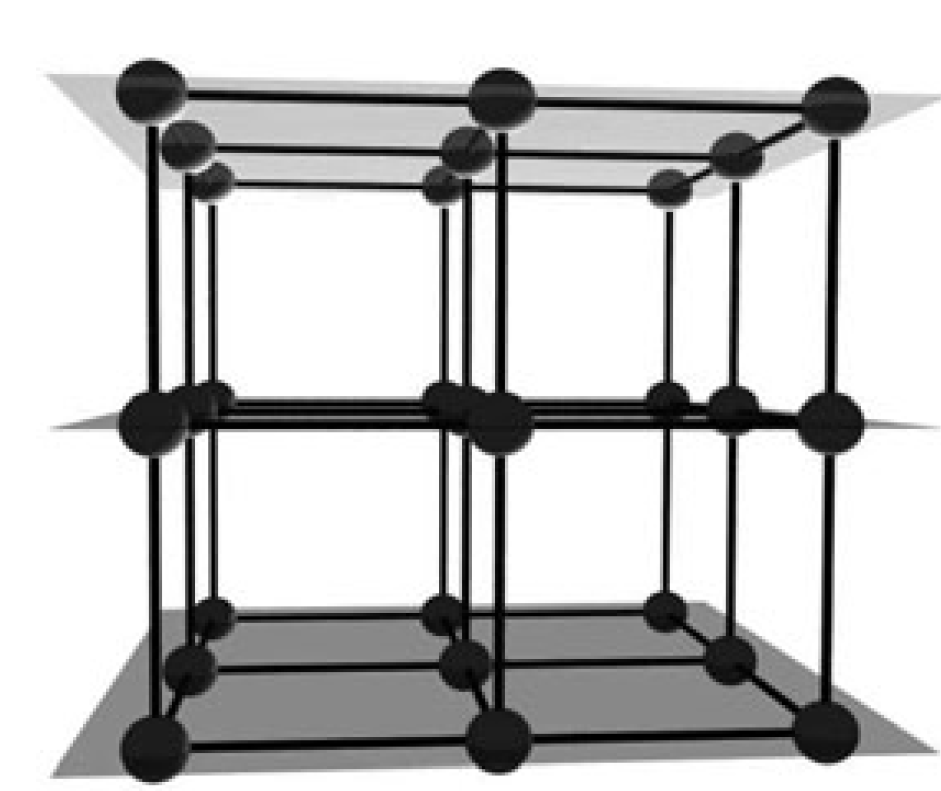
\includegraphics[scale=0.27]{Cuerpo/Ch_02/010.png}
		\caption{(010)}
	\end{subfigure}
	\begin{subfigure}{0.3\linewidth} \centering
	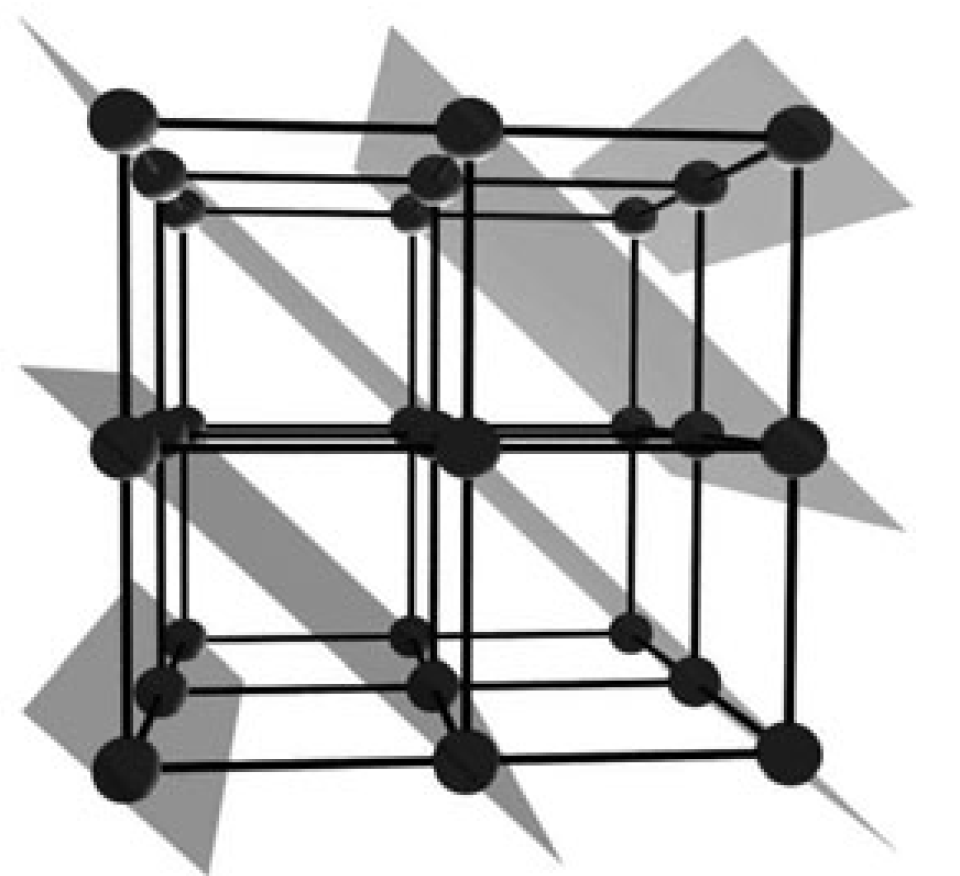
\includegraphics[scale=0.27]{Cuerpo/Ch_02/110.png}
	\caption{(110)}
	\end{subfigure}
	\begin{subfigure}{0.3\linewidth} \centering
	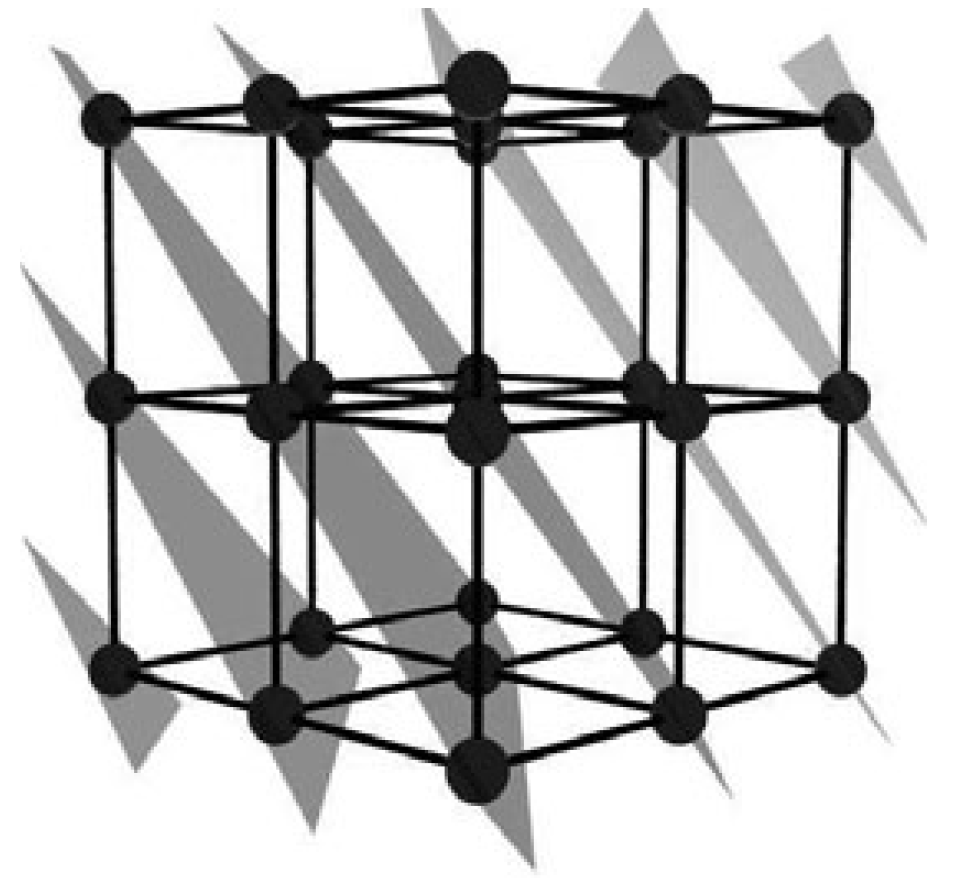
\includegraphics[scale=0.3]{Cuerpo/Ch_02/111.png}
	\caption{(111)}
	\end{subfigure}
	\caption{familias de planos reticulares para la red cúbica \sc según la notación de Miller.}
\end{figure}

Las familias de planos reticulares tienen una correspondencia uno a uno con las direcciones de los posibles vectores de la red recíproca. Esta correspondencia se debe a que \textit{los vectores de la red recíproca son normales a los planos reticulares}. Además el  \textbf{espacio entre planos reticulares} $d$ viene dado por 

\begin{equation}
	d = \frac{2\pi}{|\Gn_{\min}|} \label{Ec:02-01-06}
\end{equation}
donde $|\Gn_{\min}|$ es el \textit{vector más pequeño con dirección normal al plano}.


\subsection{Planos reticulares e índices de Miller}

Existe una notación muy interesante y útil para describir los planos reticulares, asignando a cada plano una terna (h,k,l) conocida como \textbf{índice de Miller}. Para ver cómo podemos describir un plano reticular con una terna, tenemos que empezar definiendo un vector de nuestra red recíproca como:

\begin{equation}
	G_{(h,k,l)} = h \bn_1 + k\bn_2 + l \bn_3
\end{equation}
de tal forma que $h,k$ y $l$ son siempre positivos. Dado que $\bn_i$ es un vector primitivo de la red recíproca, cada uno de las diferentes valores de h,k,l da un vector de la red recíproca diferente. Dado que para cada familia de planos reticulares existe un vector de la red recíproca existe un $\Gn$ normal a ellos, y que para cada vector de la red recíproca tenemos una terna $(h,k,l)$, podemos afirmar que a cada familia de planos reticulares le corresponde una terna. Sin embargo para $(hkl)$ deben verificar que no tienen divisores comunes, ya que de tenerlos el vector recíproco no será el vector más corto en dicha dirección y por tanto describirá una familia de planos que no contendrán puntos de red.

Este comentario es sumamente importante. Para una red cúbica (\sc, \fcc, \bcc) es conveniente elegir como los vectores $\an_i$ los vectores $a\hni,a\hnj$ y $a\hnk$ ($a$ longitud del cubo). Es decir, elegimos los vectores de la celda convencional unitaria. De esta manera los vectores $\bn_i$ son $2\pi\hni/a$,$2\pi\hnj/a$ y $2\pi\hnk/a$. Como estos vectores no son primitivos para las redes \fcc \ y \bcc, tampoco serán primitivos los vectores $\bn_i$ para la red recíproca. Esto nos lleva a que a estas redes no todos los índices de Miller ($hkl$) les corresponde una familia de planos reticulares. Esto se puede ver bien en la figura siguiente para la \bcc:

\begin{figure}[h!] \centering
	\begin{subfigure}{0.3\linewidth} \centering
		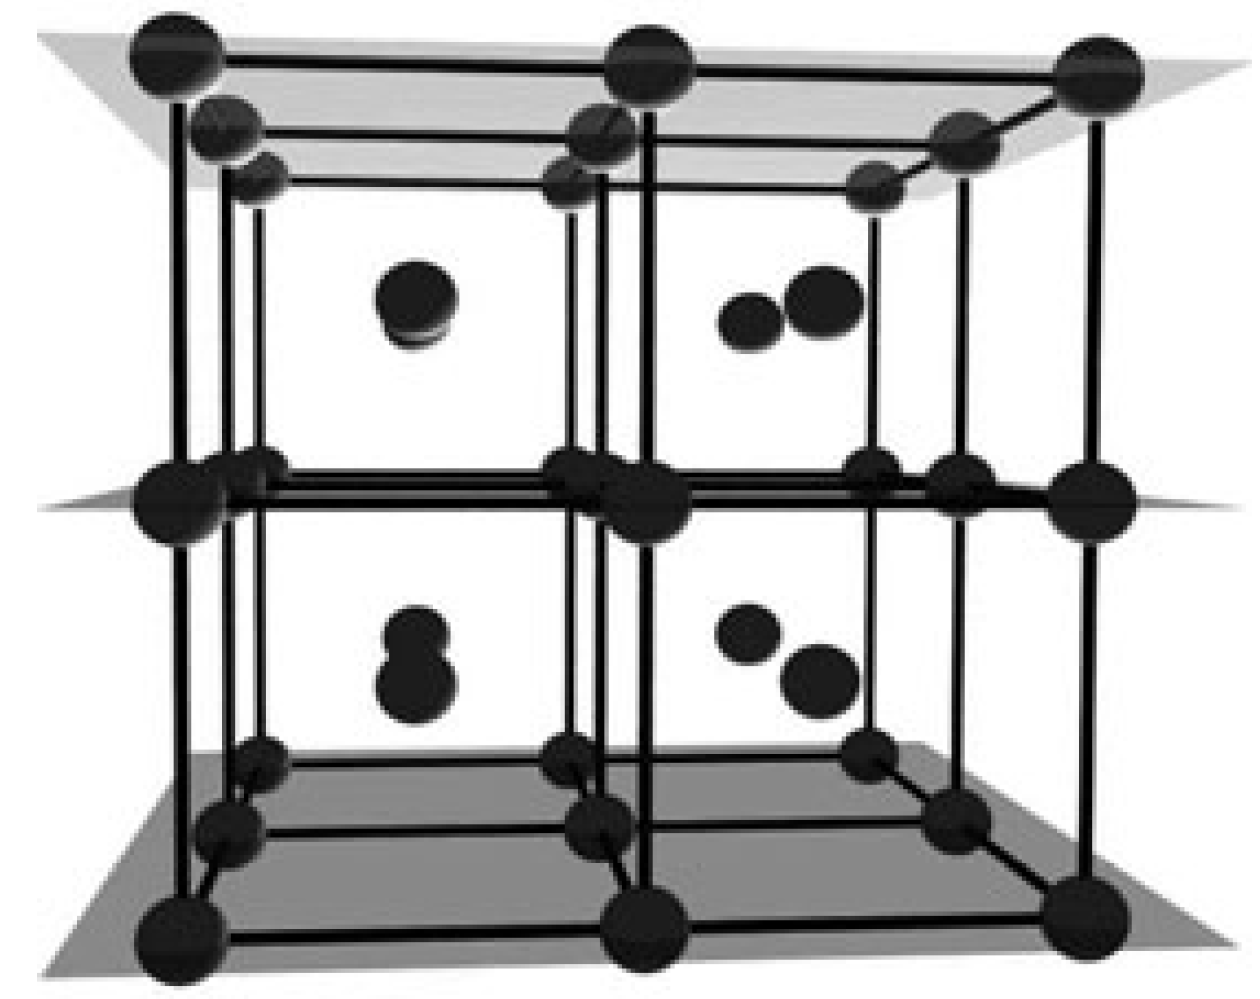
\includegraphics[scale=0.22]{Cuerpo/Ch_02/010-bcc.png}
		\caption{(010)}
	\end{subfigure}
	\begin{subfigure}{0.3\linewidth} \centering
		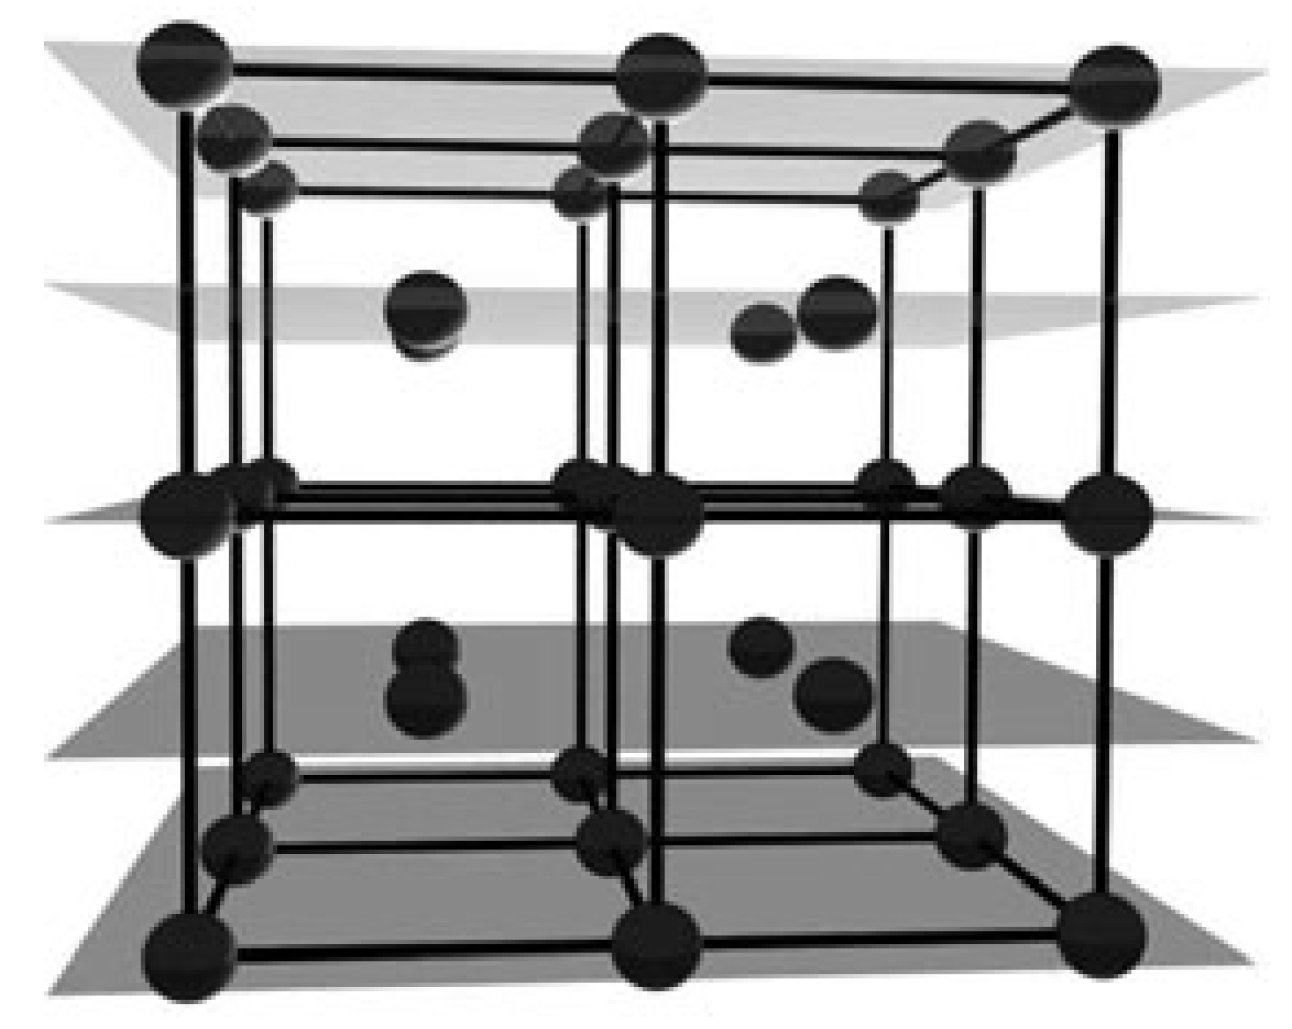
\includegraphics[scale=0.21]{Cuerpo/Ch_02/020-bcc.png}
		\caption{(020)}
	\end{subfigure}
	\begin{subfigure}{0.3\linewidth} \centering
		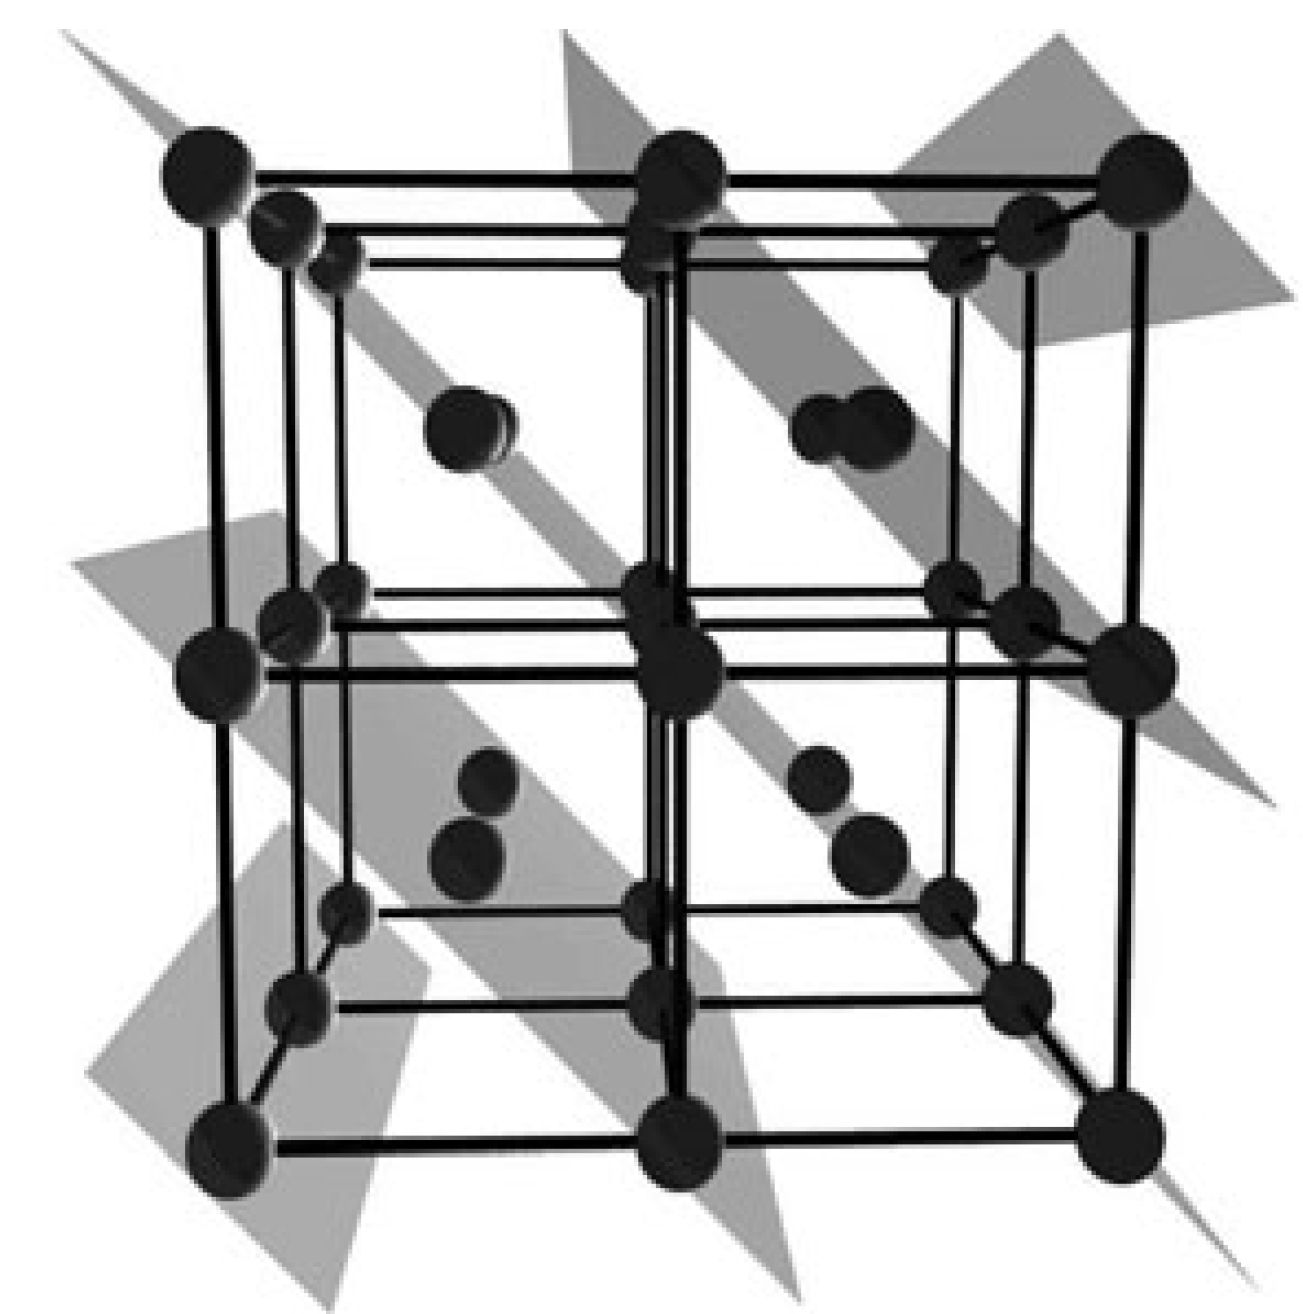
\includegraphics[scale=0.18]{Cuerpo/Ch_02/110-bcc.png}
		\caption{(110)}
	\end{subfigure}
	\caption{familias de planos reticulares para la red cúbica \bcc \ según la notación de Miller. Se puede ver que la (010) no describe adecuadamente la red \bcc.}
\end{figure}


De la ecuación \ref{Ec:02-01-06} podemos deducir que para una familia de planos reticulares definidas por los índices de Miller están separadas una distancia 

\begin{equation}
	d_{(hkl)} = \frac{2\pi}{|\Gn|} = \frac{2\pi}{\sqrt{h^2|\bn_1|^2+k^2|\bn_2|^2+l^2|\bn_3|^2}}
\end{equation}
De manera equivalente

\begin{equation}
	\frac{1}{|d_{(hkl)}|^2} = \frac{h^2}{a_1^2}+ \frac{k^2}{a_2^2}+ \frac{l^2}{a_3^2}
\end{equation}
Si $|\bn_i|=2\pi / |\an_i|$ (red cúbica) tenemos que:

\begin{equation}
	d_{(hkl)} =  \frac{a}{\sqrt{h^2 + k^2 + l^2}}
\end{equation}
Cuando hablamos del plano (200) entendemos un plano paralelo pero que corta al eje $\an_1$ en un punto distante a $a/2$ en el origen. Los índices $[uvw]$ de una dirección en un cristal son el junto de los números enteros más pequeños que poseen la relación de los componentes de un vector en la dirección deseada. En cristales cúbicos la dirección $[hkl]$ es perpendicular a un plano $(hkl)$ que posean los mismos índices, pero no es necesariamente cierto para otros sistemas cristalinos.

\begin{figure}[h!] \centering
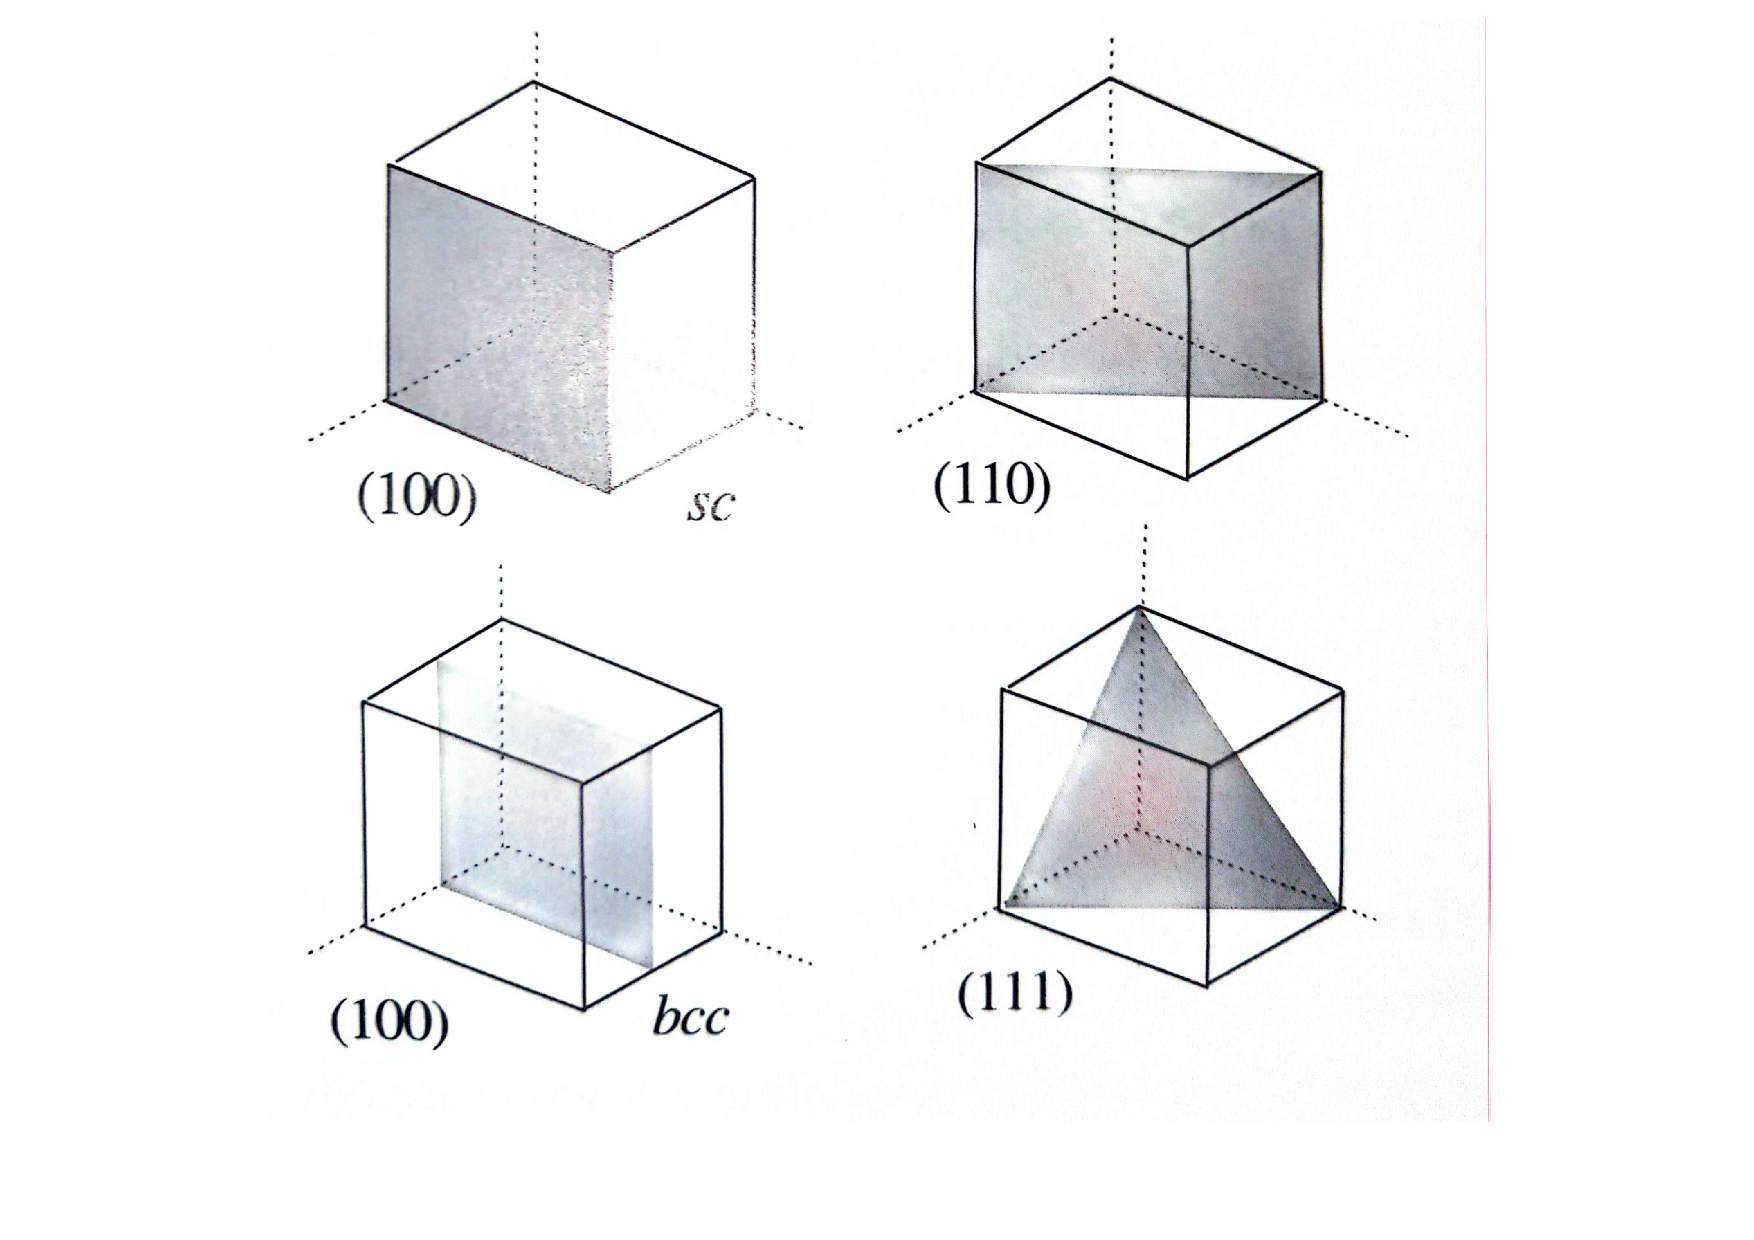
\includegraphics[scale=0.35]{Cuerpo/Ch_02/Fotos_libro 1.pdf}
\caption{Algunos planos reticulares para las redes cúbica simple (\textit{sc}) y centrada en el cuerpo (\textit{bcc}) y sus índices de Miller.}
\label{Fig:02-01}
\end{figure}

\subsection{Zonas de Brillouin} \label{Subsec:02-01-04}

Las zonas de Brillouin jugarán un papel fundamental en los temas posteriores, por lo que tener el concepto claro es fundamental, ya que nos permite describir las excitaciones del espectro de ondas en estructuras periódicas, como los cristales, por lo que será útil para poder estudiar el compartimiento del sonido, o de la luz en su interior. 

\begin{definition}
	Definimos una \textbf{zona de Brillouin} como una celda primitiva de la la red recíproca.
\end{definition}

Como se comporta el cristal bajo una onda $\kn$ permanece invariante si hacemos una trasformación del tipo $\kn \rightarrow \kn + \Gn$. De esta manera podemos darnos cuenta de que la cantidad relevante aquí es el momento cristalino, y no el momento de la onda. Por eso mismo la zona de Brillouin se ha definido de tal forma que incluye todos los momentos posibles con comportamiento diferentes entre sí (en una zona de Brilluoin cada punto $\kn$ se comporta de manera diferente a cualquier otro $\kn$ de la zona). Mientras que la la definición más general de la zona de Brillouin nos permite elegir una forma cualquiera de la celda primitiva (recordar que hay varias elecciones siempre), en general existen algún tipo de celdas mas convenientes que otras. \\

Definiremos la \textit{primera zona de Brilluoin} en el espacio recíproco de la misma manera que definimos la celda de Wigner-Seitz en la red directa. 

\begin{definition}
	Comenzando por un punto de la red recíproca $\Gn=0$, todos los $\kn$ que están mas cerca a $\mathbf{0}$ que de cualquier otro punto de la red recíproca decimos que se encuentran en la \textbf{primera zona de Brilluoin}. De manera parecida, todos los puntos $\kn$ que su segundo punto más cercano es el $\mathbf{0}$, decimos que pertenece a la \textbf{segunda zona de Brillouin}. De manera análoga podemos definir la tercera, cuarta... zona de Brilluoin.  \label{Def:02-05}
\end{definition}

Al igual que la celda de Wigner-Seitz, existe un algoritmo simple para construir las zonas de Brilluoin. Dibuja las líneas entre los vecinos, y traza una línea perpendicular en el punto mitad entre ambos vecinos. Estas bisectrices formarán las fronteras de las zonas de Brillouin. Cualquier punto que puedas obtener desde el $\mathbf{0}$ hasta una de las fronteras es un vector de la primera zona de Brilluoin (véase imagen \ref{Fig:02-03-1a}). La construcción de la primera zona de Brilluoin análoga a la la celda de Wigner-Seitz.

\begin{figure}[h!] \centering
	\begin{subfigure}{0.45\linewidth} \centering
		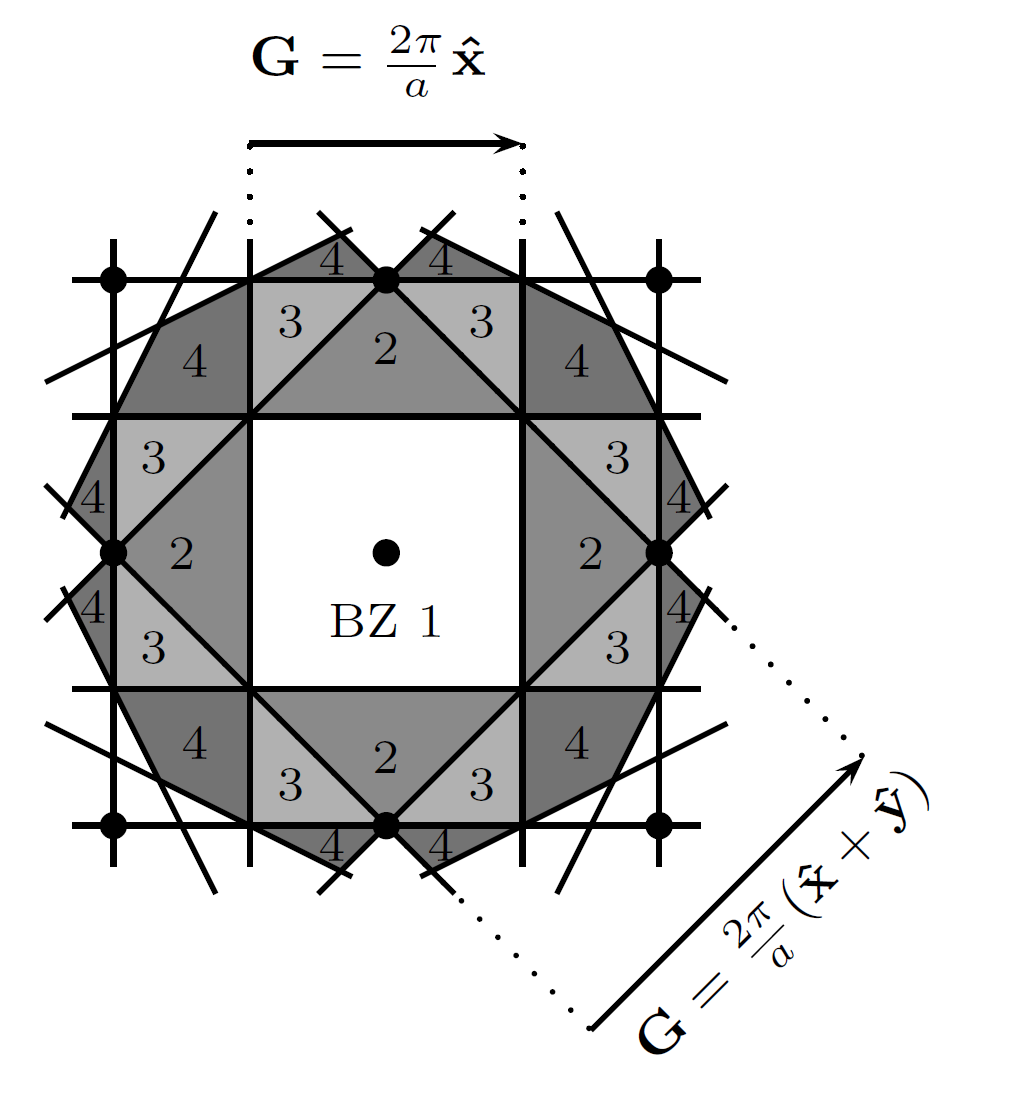
\includegraphics[scale=0.3]{Cuerpo/Ch_02/Brillouin.png}
		\caption{zonas de Brilluouin red cuadrada.} \label{Fig:02-03-1a}
	\end{subfigure}
	\begin{subfigure}{0.45\linewidth} \centering
	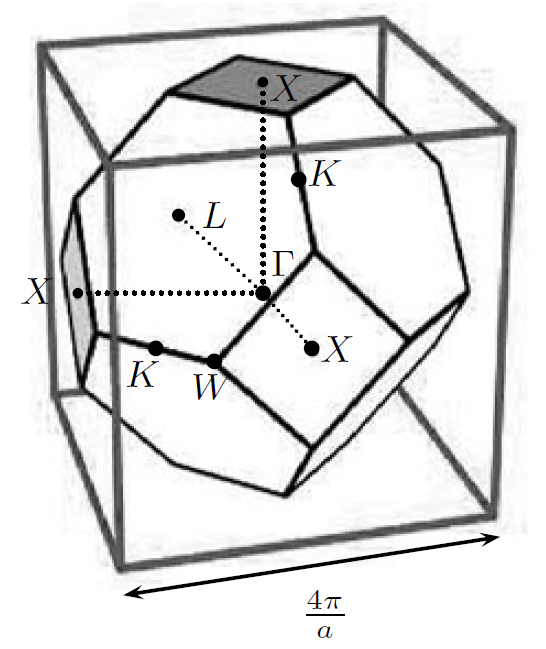
\includegraphics[scale=0.45]{Cuerpo/Ch_02/Brillouin-bcc.png}
	\caption{primera zona de Brillouin de la red \fcc.}
	\end{subfigure}
	\caption{}
\end{figure}

\section{Difracción}

Sea una onda plana $e^{\kn \cdot \rn}$ incidente sobre un cristal. En esta sección queremos estudiar cual es la dirección de la onda dispersada para la que tenemos un máximo de difracción. Supongamos que la amplitud de la onda dispersada en la dirección $\kn'$ (ver figura \ref{Fig:02-02}) suponiendo \textit{dispersión elástica} $(|\kn|=|\kn|')$. En ese caso la amplitud de la onda (la intensidad es $I\propto A^2$) vendrá dada por 

\begin{equation}
    A_{\text{salida}} \propto \sum_{m,n} f_{mn} e^{i \Delta \phi_{mn}}
\end{equation}
siendo $\Delta \phi_{mn} = (\kn - \kn') \cdot \dn_{mn}$ la diferencia de fase entre la onda reemitida por un centro dispersor ($m$) y otro ($n$) a una distancia $\dn_{mn}$ del primero. La suma ($m,n$) a todos los centros dispersores puede hacerse sumando a todas las celdas en \textit{posiciones de red} $\Rn_n$ y a todos los átomos de la base en posiciones $\rn_j$ dentro de cada celda, tal y como se puede ver en la figura \ref{Fig:02-03}. Entonces esta distancia vendrá dada por $\dn_{mn}=\Rn_n+\rn_j$ con lo que la amplitud de onda viene dada por:

\begin{equation}
    A_{\text{salida}} \propto  \sum_{n,j} f_j e^{-i (\Rn_n + \rn_j) \cdot \Delta \kn} = \sum_j^{\text{base}} f_j e^{-i \rn_j \cdot \Delta \kn} \sum_{n}^{\text{red}} e^{-i\Rn_n \cdot \Delta \kn} \label{Ec:02-02-02}
\end{equation}
con $\Delta \kn = \kn' - \kn$. A $f_j$ es el llamado \textit{factor de forma atómico}, que da cuenta del distinto \textit{poder dispersor} de los átomos de la base. El máximo de $A_{\text{salida}}$ lo marca el segundo factor que suma a toda la red, pues es una suma del orden de $10^{23}$ términos frente a unos pocos del primero. \\

En cualquier caso no podemos despreciar este primer término, ya que de hacerse cero para alguna onda o dirección de onda, se anularía la amplitud de salida. Esto se estudiará en la siguiente sección \ref{Sec:02-03}. El máximo se alcanza con la condición de que

\begin{equation}
    \Delta \kn \cdot \Rn_n = 2 \pi \times \text{entero} \label{Ec:02-02-03}
\end{equation}
para cualquier vector de red $\Rn_n$. La interpretación es que todas las celdas (son las celdas las que están conectadas por vectores de red) deben reemitir en fase para que la suma sea máxima (ver figura \ref{Fig:02-04}, solo con la interferencia constructiva hay máximo).    


La condición (\ref{Ec:02-02-03}) para $\Delta \kn$ implica precisamente que para que haya un máximo $\Delta \kn$ \textit{debe ser un vector de la red recíproca}. Así pues, el resultado básico es que para que haya máximo de difracción (interferencia constructiva) se debe satisfacer 
\begin{equation}
    \Delta \kn = \Gn\label{Ec:02-02-04}
\end{equation}
que también lo podemos expresar como 

\begin{equation*}
	\kn' = \kn + \Gn
\end{equation*}
Elevando la ecuación (\ref{Ec:02-02-04}) al cuadrado y teniendo en cuanta que $|\kn|=|\kn'|$ es inmediato ver que esta condición se puede escribir en función del vector de ondas de la radiación incidente y de los vectores de la red recíproca del cristal: 

\begin{equation*}
	2\kn \cdot \Gn + |\Gn|^2 = 0
\end{equation*}
Reemplazando $\Gn$ por $-\Gn$ en esta expresión, la condición de difracción es: 

\begin{equation}
    2 \kn \cdot \Gn = |\Gn|^2 \Longleftrightarrow \kn \cdot \hat{\Gn} = \frac{1}{2} |\Gn| \label{Ec:02-02-05}
\end{equation}
y la dirección en la que se observa el máximo es entonces $\kn'=\kn-\Gn$. 


Llamando \textit{plano Bragg} a aquel que es mediatriz a cualquier vector de red de la red recíproca, la interpretación de (\ref{Ec:02-02-05}) es que la difracción ocurre para los índices $\kn$ incidentes tales que, con origen en un punto cualquiera de la red recíproca, su extremo caiga sobre un plano de Bragg (figura \ref{Fig:02-05}). En particular, lo anterior es válido para la frontera de la \textit{PZB}\footnote{\textit{PZB} $\equiv$ Primera zona de Brilluoin. Véase definición \ref{Def:02-05}.} por estar formada por planos de Bragg. 

\begin{figure}[h!]\centering
\begin{subfigure}{0.43\linewidth} \centering
	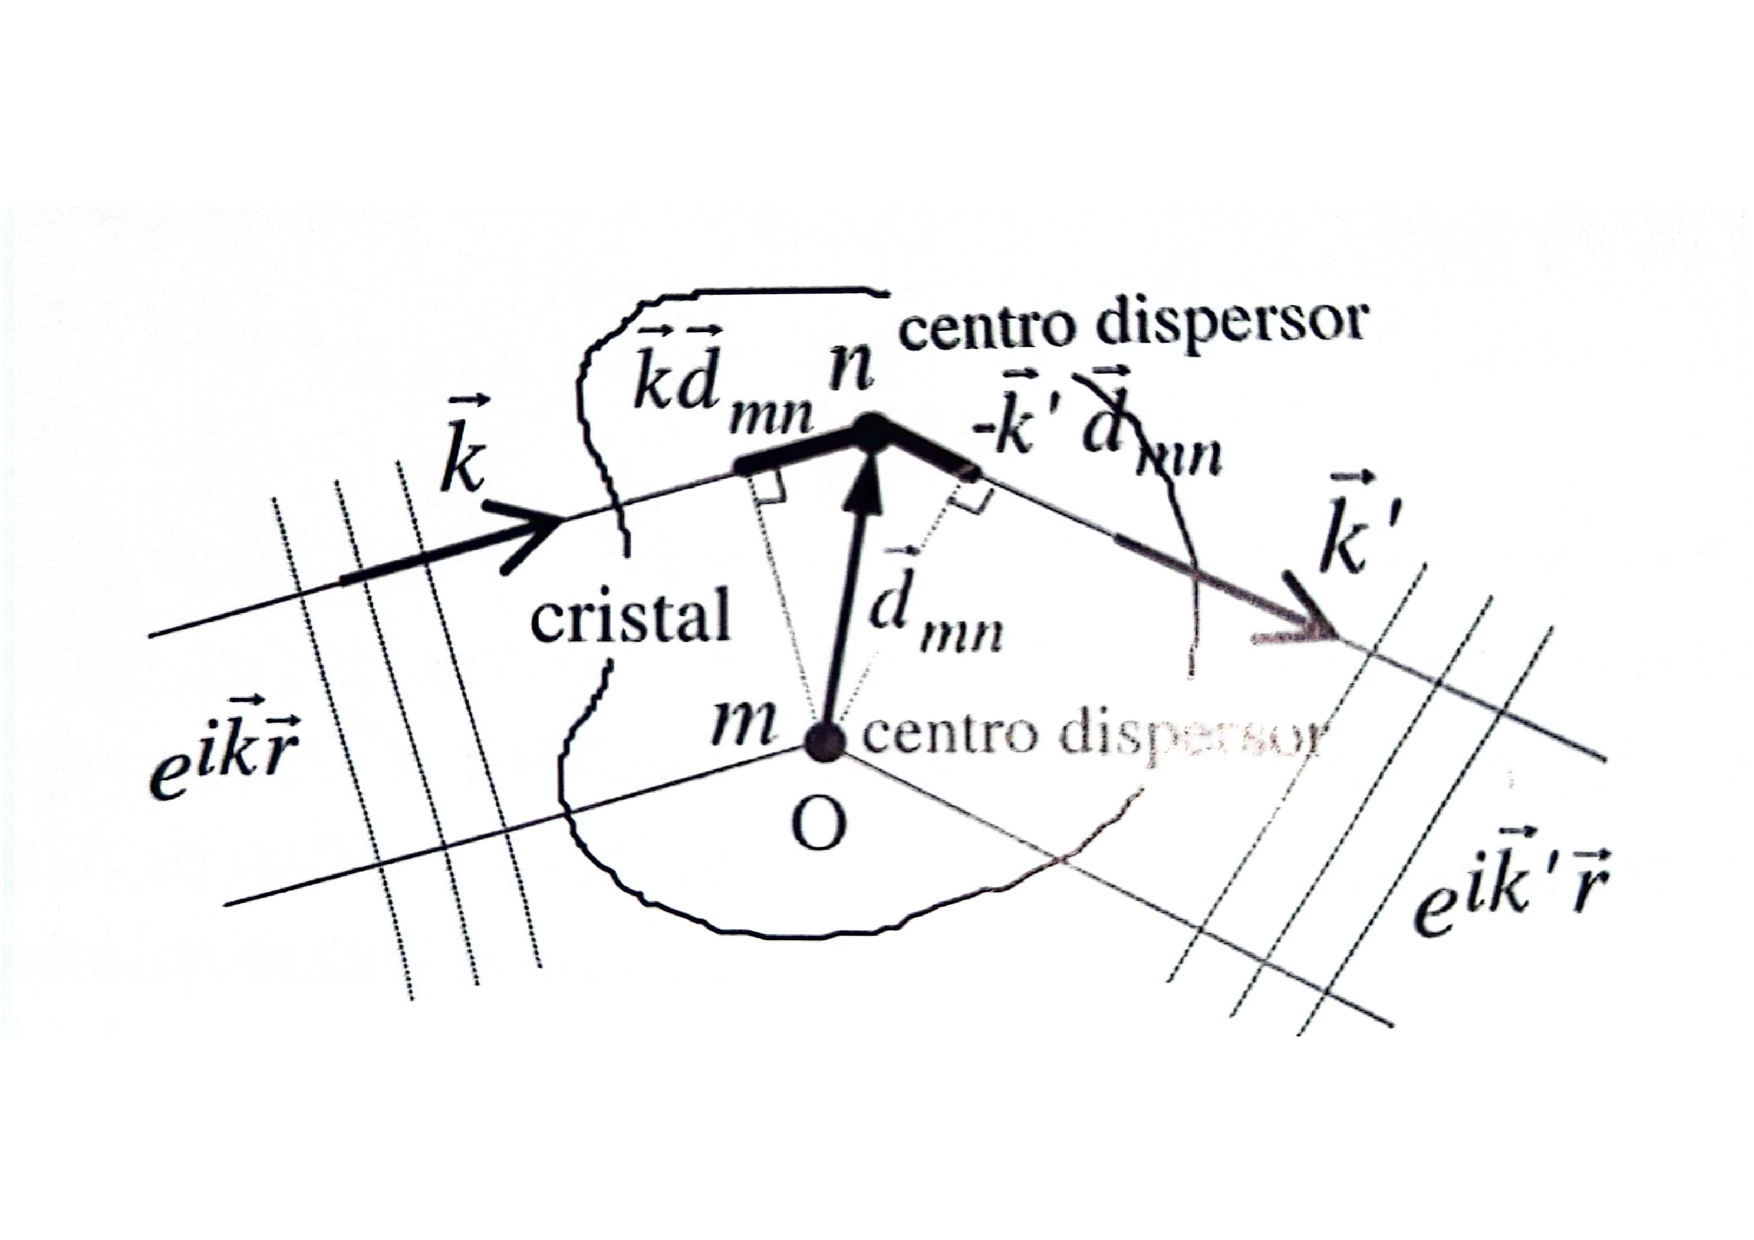
\includegraphics[scale=0.30]{Cuerpo/Ch_02/Fotos_libro 2.pdf}
	\caption{Diferencia de camino recorrido por las ondas dispersadas por dos centros m,n separados $\dn_{mn}$.}
	\label{Fig:02-02}
\end{subfigure}
\begin{subfigure}{0.43\linewidth} \centering
	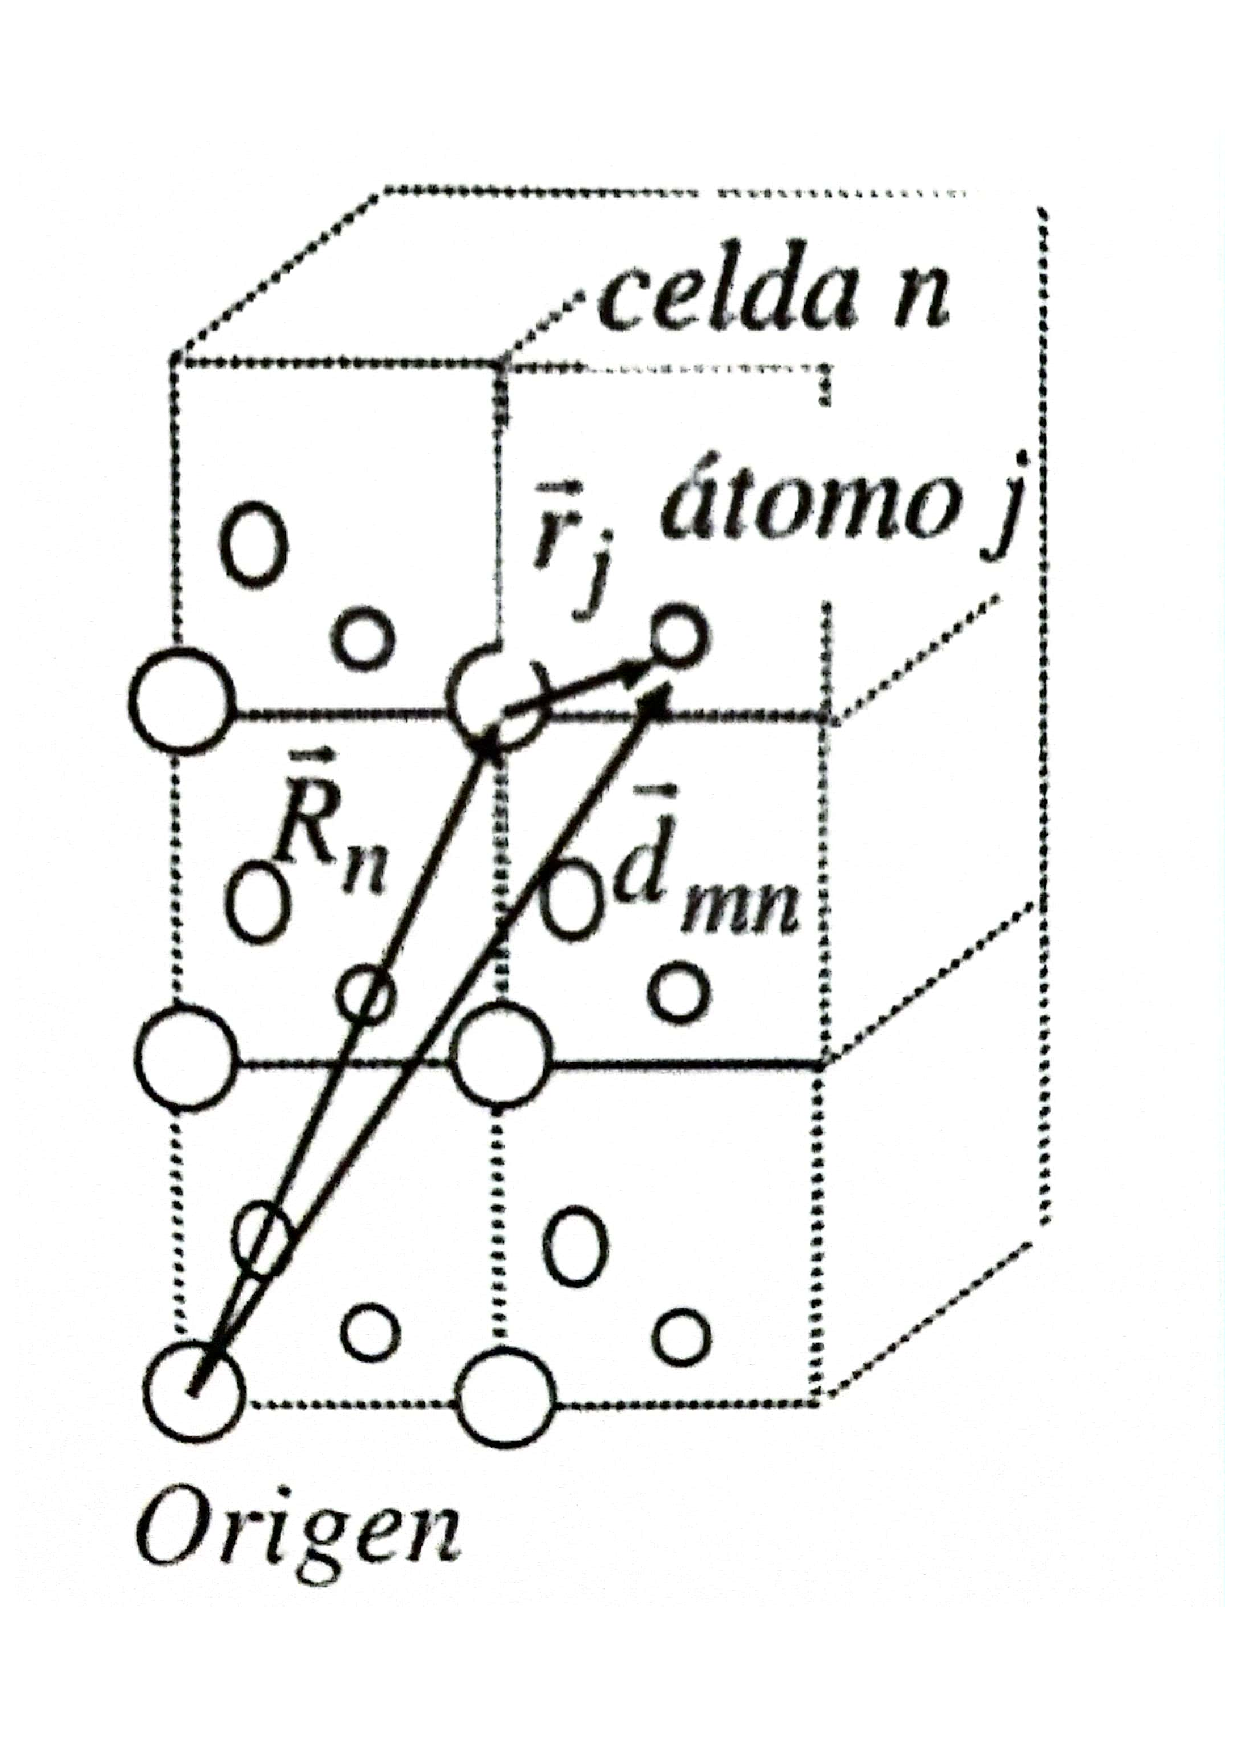
\includegraphics[scale=0.20]{Cuerpo/Ch_02/Fotos_libro 3.pdf}
	\caption{Posición de los centros dispersores de cada celda $n$ en posición $\Rn_n$.}
	\label{Fig:02-03}
\end{subfigure}
\caption{}
\end{figure}


\begin{figure}[h!]\centering
\begin{subfigure}{0.43\linewidth} \centering
	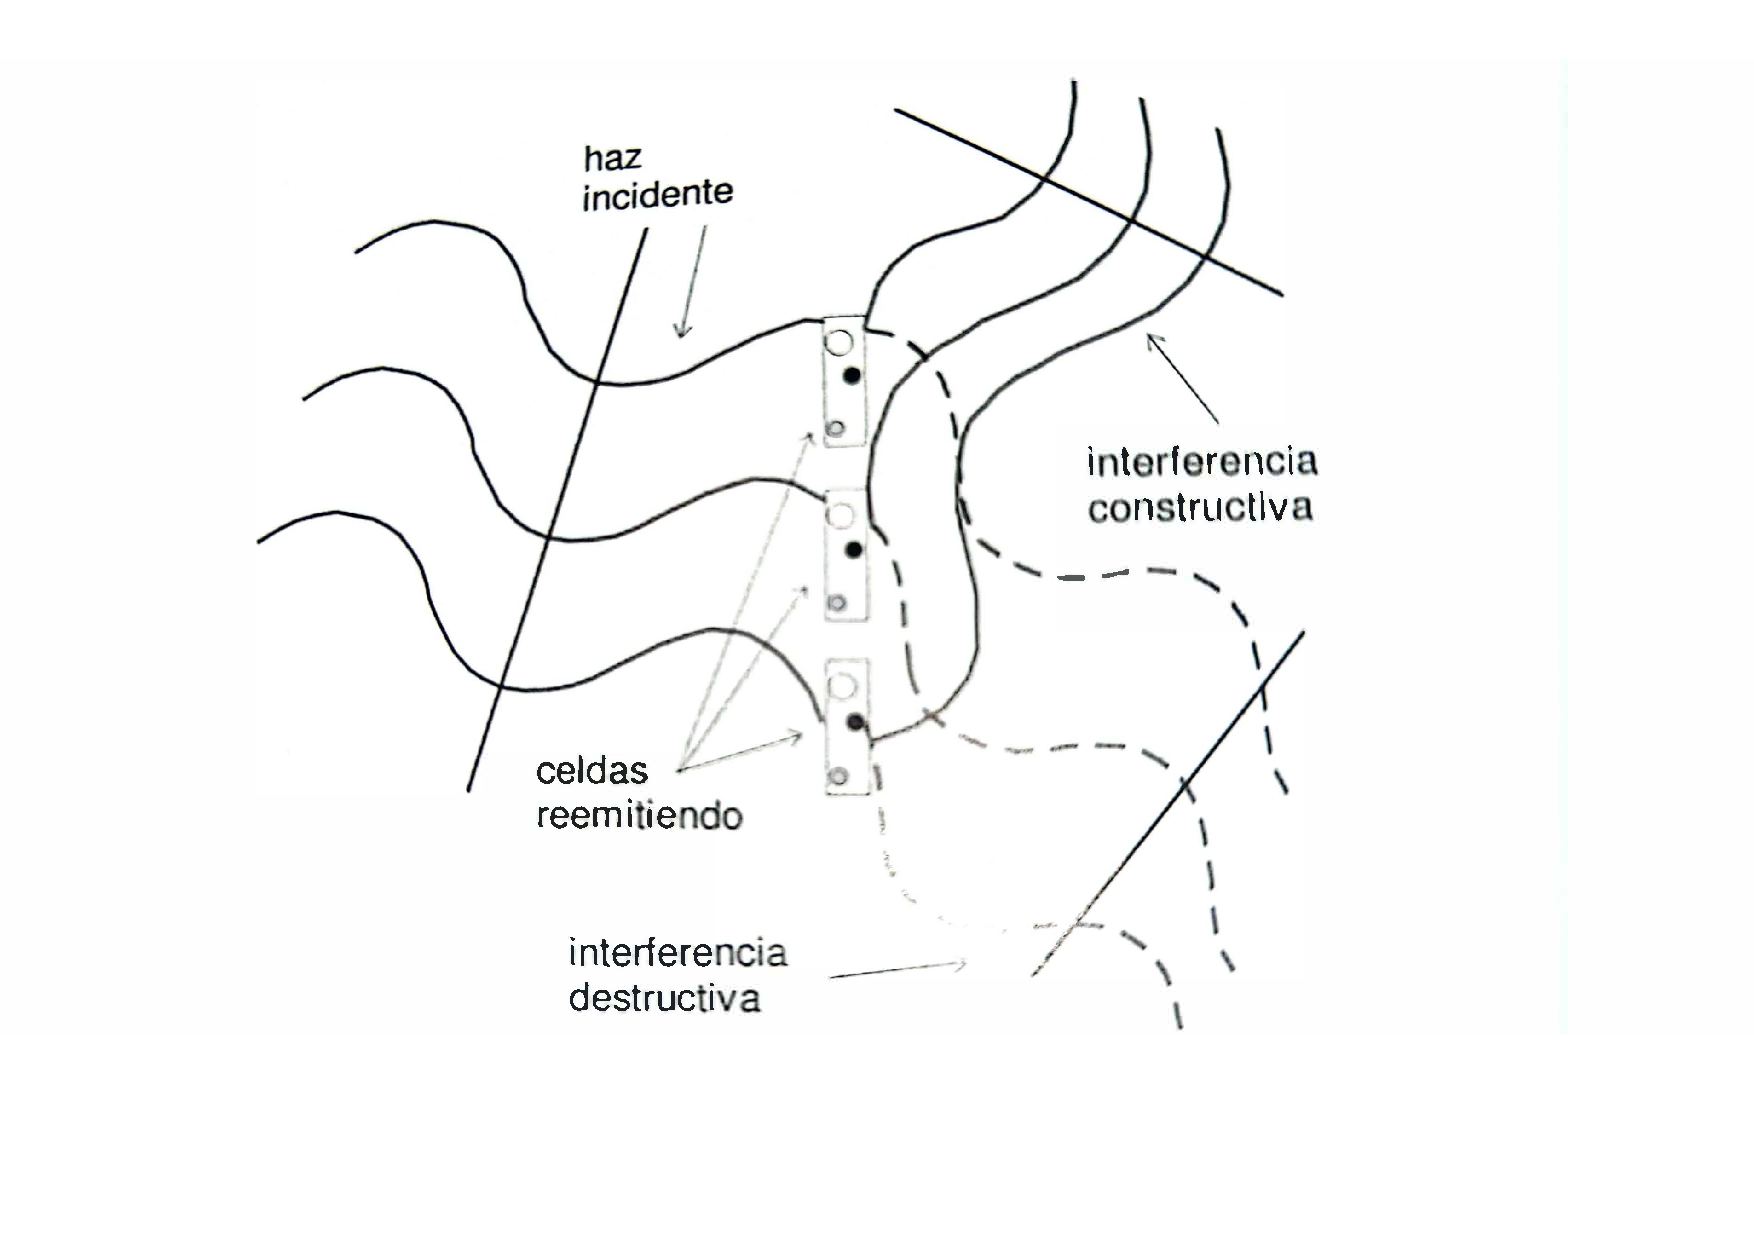
\includegraphics[scale=0.25]{Cuerpo/Ch_02/Fotos_libro 4.pdf}
	\caption{Reemisión de las celdas en fase o no según la dirección considerada}
	\label{Fig:02-04}
\end{subfigure}
\begin{subfigure}{0.43\linewidth} \centering
    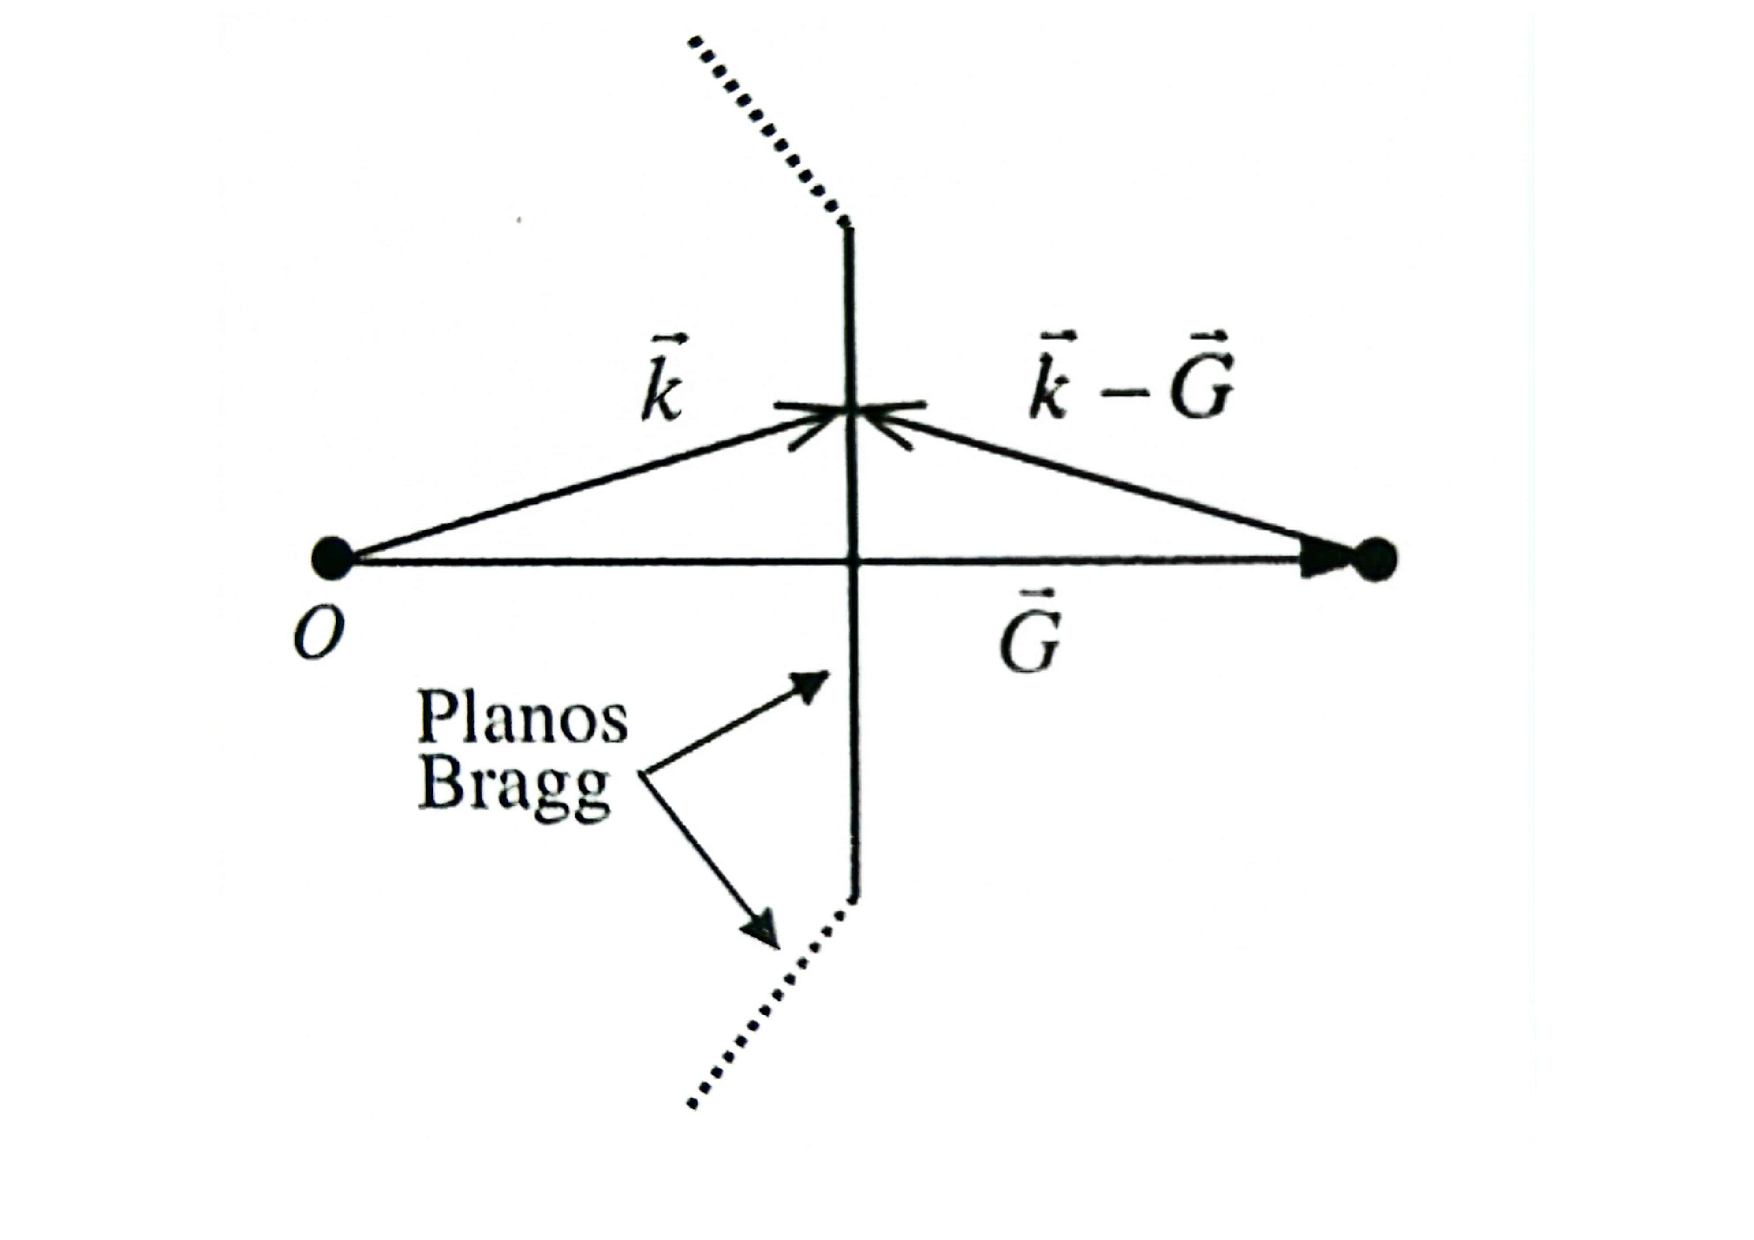
\includegraphics[scale=0.24]{Cuerpo/Ch_02/Fotos_libro 5.pdf}
    \caption{Equivalencia geométrica de la condición de difracción dada por la Ec. \ref{Ec:02-02-05}.}
    \label{Fig:02-05}
\end{subfigure}
\caption{}
\end{figure}

\subsection{Ley de Bragg}

Otra formulación equivalente de la condición de difracción es la llamada \textbf{ley de Bragg} (1913), que admite que la radiación sufre una reflexión especular en los distintos planos reticulares (figura \ref{Fig:02-06}) de modo que sólo si las reflexiones de dos sucesivos planos están en fase se observará máximo de difracción. Es muy fácil de ver que la diferencia de caminos entre planos sucesivos es de $2d\sin \theta$ por lo que esta cantidad deberá ser múltiplo entero de longitudes de onda $\lambda$, es decir,

\begin{equation}
    n \lambda = 2 d \sin (\theta) \label{Ec:02-02-06}
\end{equation}
La equivalencia de la ley de Bragg (ecuación \ref{Ec:02-02-06}) con la formulación más general de las ecuaciones \ref{Ec:02-02-03} y \ref{Ec:02-02-04} se deduce de la correspondencia vista entre vectores de la red recíproca y sistemas de planos reticulares. En efecto, el vector $\Gn$ a que hace referencia (\ref{Ec:02-02-04}) de componentes ($h' k' l'$) no necesariamente primos entre sí, verifica $G=2k\sin \theta$ (figura \ref{Fig:02-07}). Sea ahora $\Gn_0$ el vector de la red recíproca paralelo a $\Gn$ más corto, que debe tener componentes ($hkl$) primas entre sí (por no haber otro más corto), y que verifica $\Gn = n \Gn_0$ (en componentes $h'=nh$, $k'=nk$, $l'=nk$). Como $G_0 = 2\pi/d$ (ecuación \ref{Ec:02-01-06}), al sustituir resulta $n2\pi/d=2k\sin (\theta) \Rightarrow n \lambda = 2 d \sin (\theta)$. 
\begin{figure}[h!] \centering
\begin{subfigure}{0.43\linewidth} \centering
    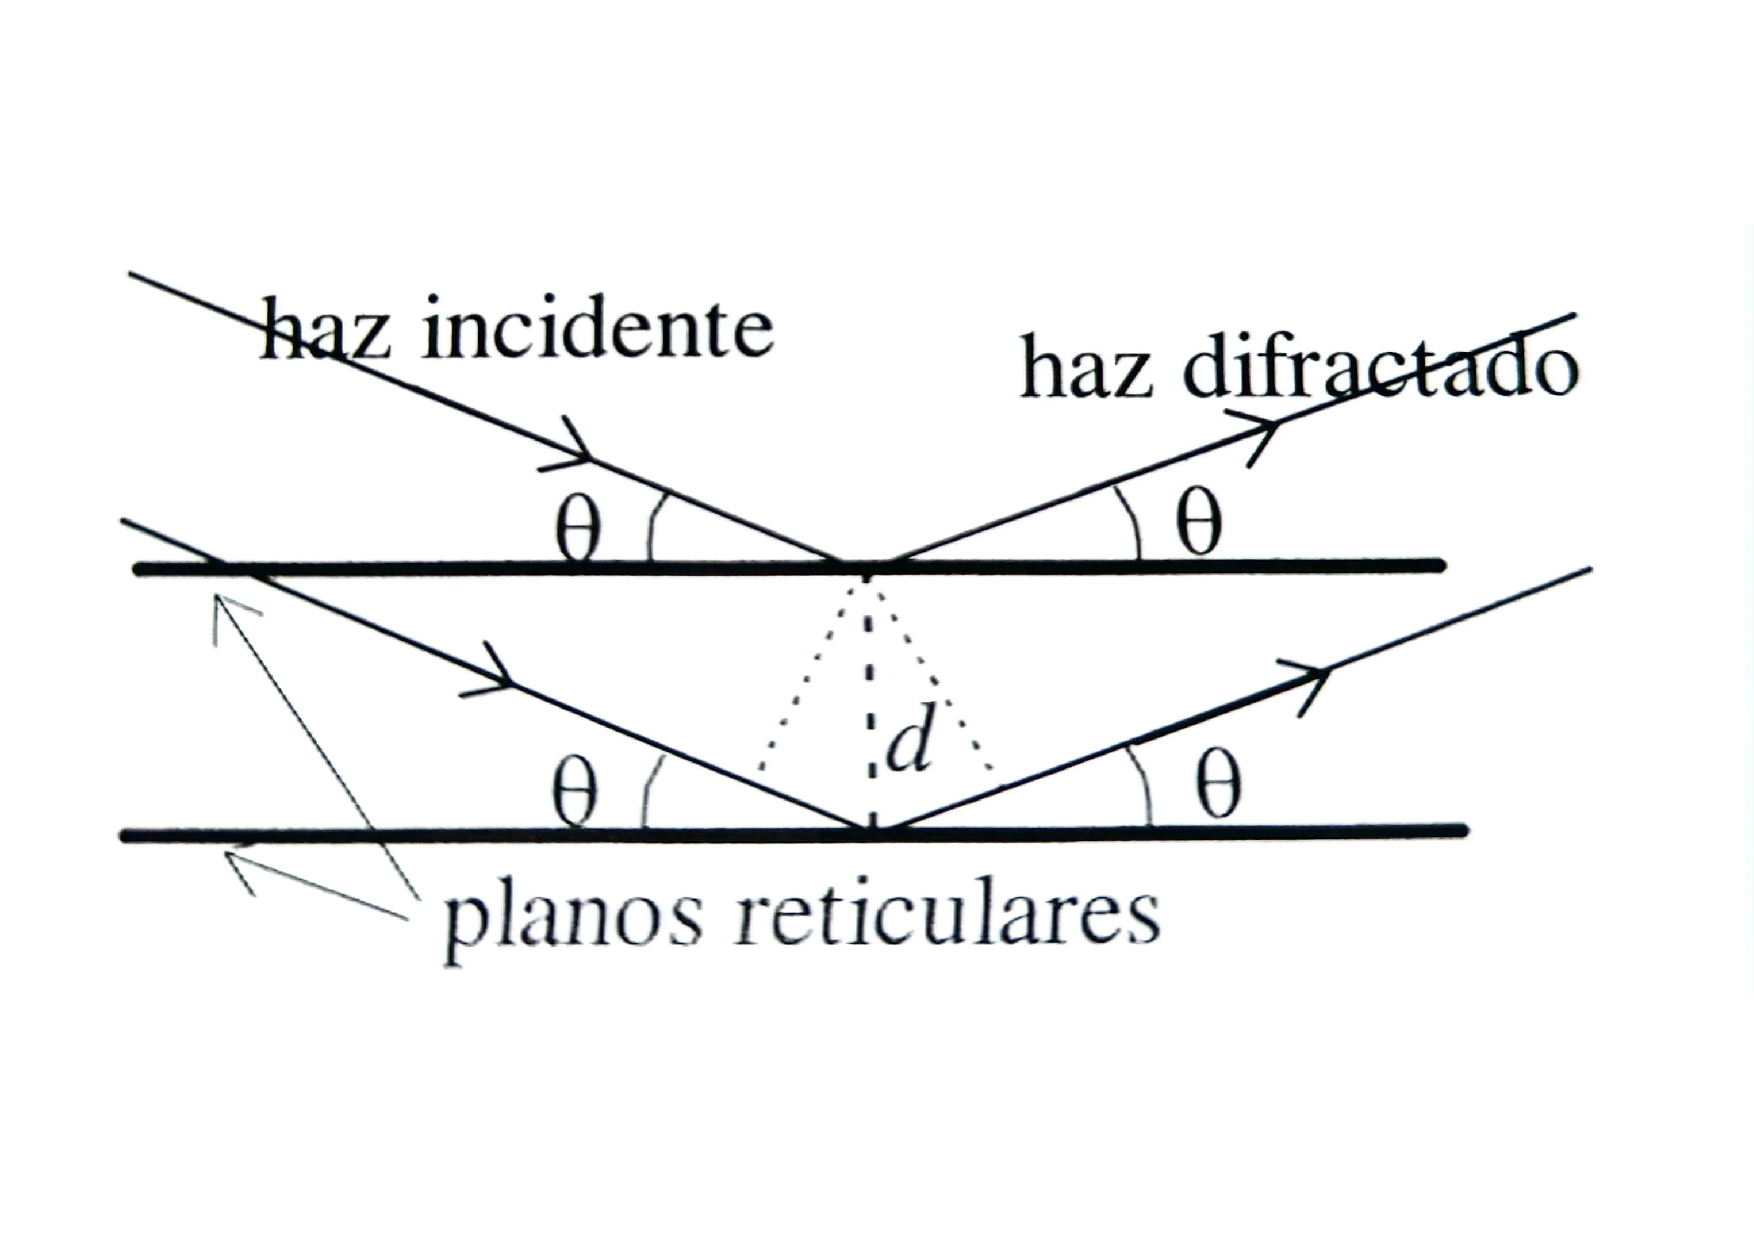
\includegraphics[scale=0.3]{Cuerpo/Ch_02/Fotos_libro 6.pdf}
    \caption{Diferencia de camino recorrido por los haces reflejados especularmente por dos planos reticulares consecutivos.}
    \label{Fig:02-06}
\end{subfigure}    
\begin{subfigure}{0.43\linewidth} \centering
    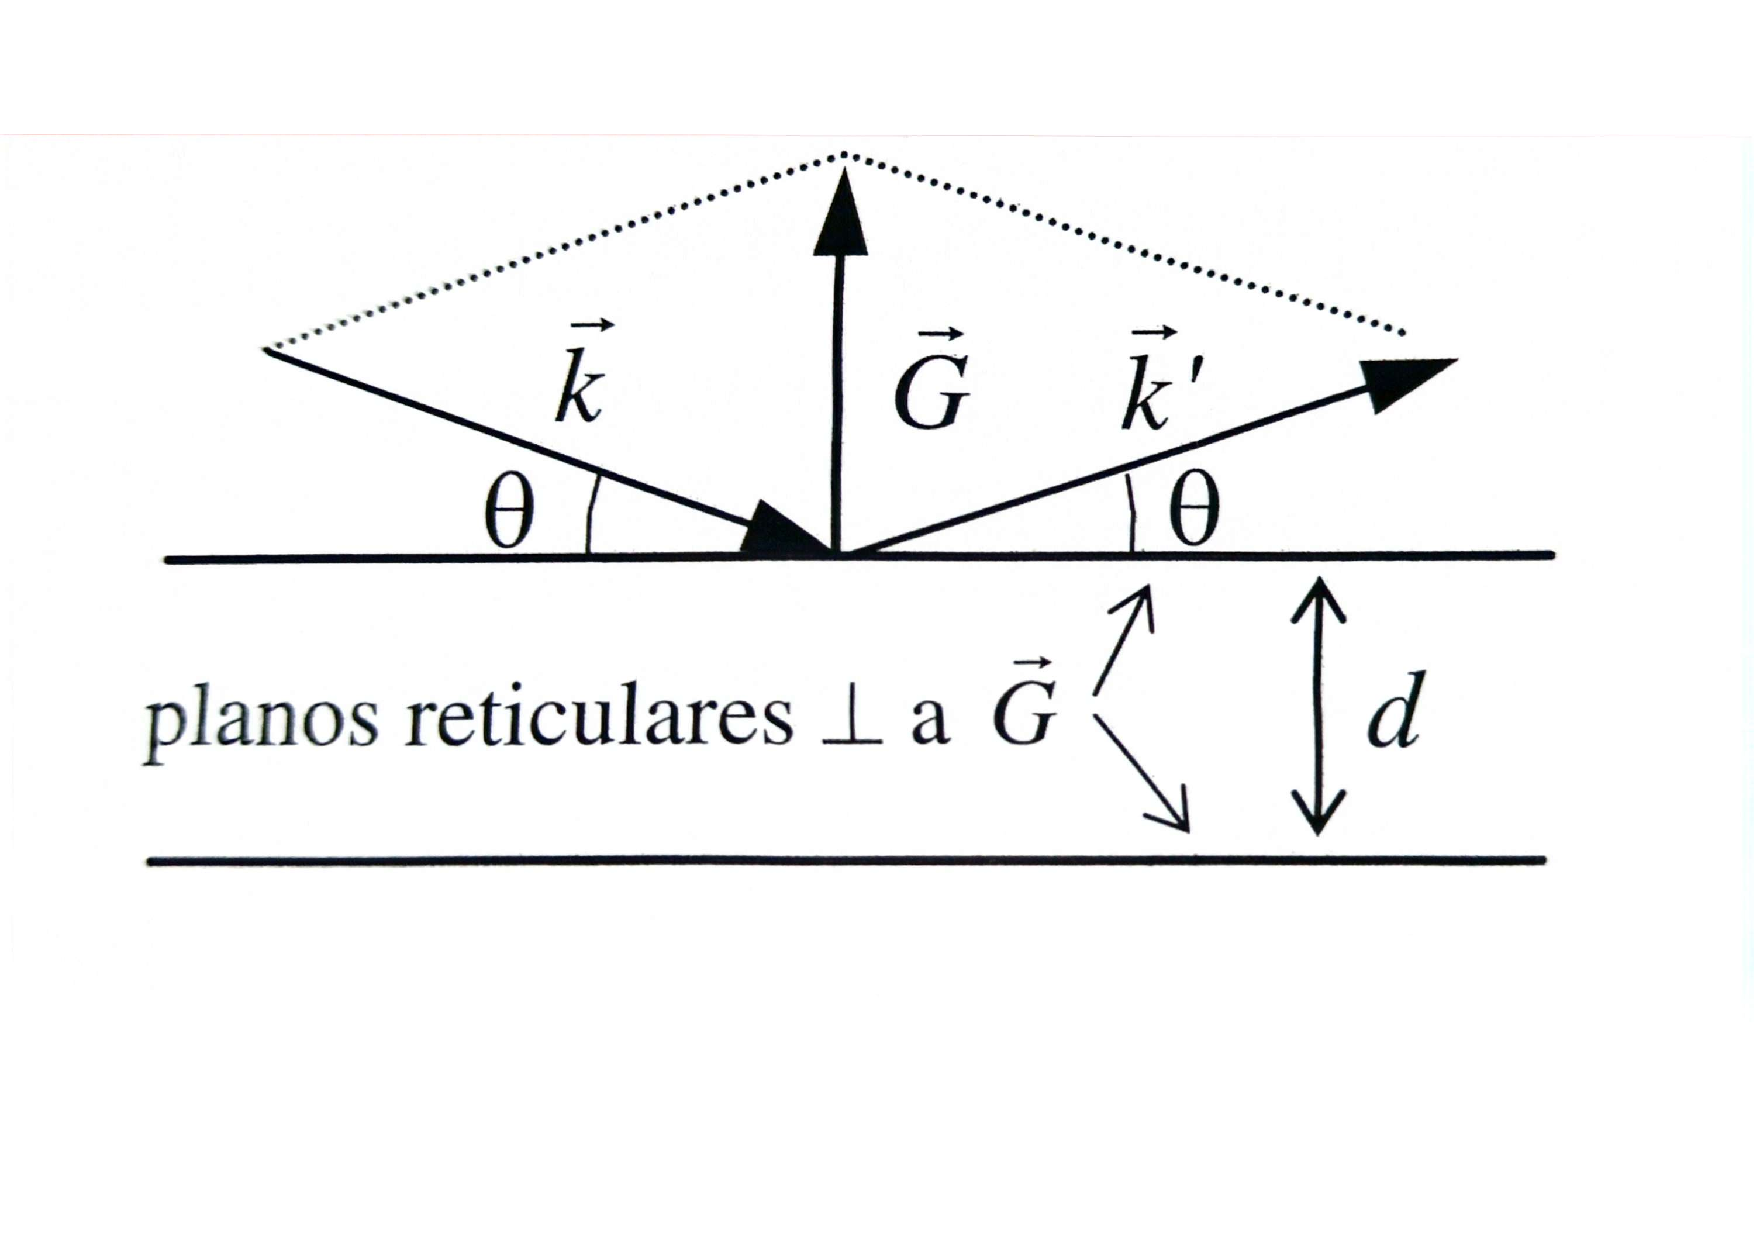
\includegraphics[scale=0.3]{Cuerpo/Ch_02/Fotos_libro 7.pdf}
    \caption{Correspondencia entre vectores de la red recíproca $\Gn$ y sistemas de planos de la red directa.}
    \label{Fig:02-07}
\end{subfigure}
\caption{}
\end{figure}


\section{Factor de estructura} \label{Sec:02-03}

Como hemos dicho, no solo hay que tener en cuenta la dispersión por los centros de red, si no que también hay que tener en cuenta la dispersión cada celda de la red. Aunque las celdas estén en fase entre sí, si debido a la interferencia entre los átomos de cada celda estas no emiten, no habrá máximo de intensidad. Esto tendrá que ver con el concepto \textit{reglas de selección} que introduciremos más tarde. 

Ahora queremos precisar ahora la intensidad de los distintos máximos de difracción. En condición de máximo, la amplitud dispersada (dirección $\hnk'$) es por \ref{Ec:02-02-02} y \ref{Ec:02-02-03}, viene dada por 

\begin{equation}
    A_{\text{salida}} \propto N \sum_j^{\text{base}} f_j e^{-i\rn_j \cdot \Delta \hnk} = N S_{\Gn} \label{Ec:02-03-01}
\end{equation}
siendo $N$ el número de celdas. El sumatorio denotado por $S_\Gn$ representa una \textit{suma interferencial dentro de una celda} y se denomina \textbf{factor de estructura de la base}, que a su vez depende del \textbf{factor de estructura atómico} que representamos por $f_j$. y del \textit{número de átomos y tipo de átomos de la base}. Impuesta la condición de máximo de red tendríamos que

\begin{equation}
	S_{\Gn} = \sum_{j}^{\text{base}} f_j e^{i \rn_j \cdot \Gn} \label{Ec:02-03-02}
\end{equation}

\subsection{Factor de estructura atómico}

El factor de forma del átomo genérico $f_j$, a su vez, no es sino una suma interferecnial interna (intraatómica). 

\begin{equation}
	f_j = \int n_j (\rn) e^{-i \rn \cdot \Gn} \D^3 \rn
\end{equation}
siendo $n_j (\rn)$ la concentración electrónica en el elemento de volumen atómico $\D^3 \rn$ del átomo $j$, y donde ya se ha supuesto condiciones de máximo de difracción ($\Delta \kn  = \Gn$). El factor de forma atómico, obtenido de la difracción de rayos x da información de la distribución atómica, observándose diferencias de sólo unos pocos por ciento respecto de los valores teóricos de los átomos libres. 
 
\subsection{Factor de estructura para bases poliatómicas}

El factor de estructura atómico contiene una información muy relevante acerca de la estructura atómica. Sin embargo, no contiene nada de información acerca de como es la red (el factor de red $a$, si es una \fcc, \bcc...). Sin embargo el factor de estructura de la base también depende de la disposición de la red. Para esto tenemos que recordar que las redes cúbicas $\fcc$ y $\bcc$ pueden ser descritas como $\sc$ pero con bases poliatómicas. Por ejemplo, la $\bcc$ es una $\sc$ con una base diatómica tal que se encuentran en [0,0,0] y [a/2,a/2,a/2].  

Como ya hemos dicho, esto hará que para ciertos máximos de difracción permitidos por la red estén prohibidos por la base atómica ($S_\Gn=0$), lo que proporciona una valiosa información sobre su estructura. A las condiciones que deben verificarse  para que no se anulen las llamamos \textbf{reglas de selección}. Como se puede ver en \ref{Ec:02-03-02}, dado que para que haya máximos $\Delta \kn$ debe ser un vector de la red recíproca, y este a su vez puede ser expresado como una terna de ($h,k,l$), tendremos que podremos expresar las reglas de selección diciendo que el vector de onda máximo de red ($h,k,l$) es o no es válido. Las condiciones para que se anulen:

\begin{table}[h!] \centering
	\begin{tabular}{l|l}
		Red & Condiciones \\ 
		\hline 
		\sc & No se anula nunca. \\
		\bcc & $h+k+l$ deben de ser impar. \\
		\fcc & En $h,j,l$  un termino debe tener diferente paridad a los otros dos. \\
		Diamante & (Regla \fcc)  o ($h+k+l=2+4n$ con $n$ entero) \\
	\end{tabular}
\end{table}

\subsection{Cálculo de reglas de selección}

A continuación veremos como calcular las reglas de la \bcc, la \fcc \ y la estructura diamante.

\subsubsection{Reglas de selección \bcc}

Consideremos un cristal de un átomo $Z$ con estructura \bcc. La estructura \bcc puede ser descrita como una \sc \ con dos átomos en las posiciones [0,0,0] y [a/2,a/2,a/2]. En ese caso calculamos $S_{\Gn}$:

\begin{equation*}
	S_{\Gn} = \sum_{j}^{\text{base}} f_Z e^{i \rn_j \cdot \Gn}  = f_Z \parentesis{1+e^{i 2 \pi (h/2+k/2+l/2)} } =  f_Z \parentesis{1+e^{i \pi (h+k+l)} } = f_Z (1+(-1)^{h+k+l})
\end{equation*}
Como podremos ver, no habrá máximo de difracción cuando el interior del paréntesis se anule, esto es que $h+k+l$ sea un número impar. En otras palabras, \textit{habrá máximo de difracción cuando $h+k+l$ sea par}. 

Lógicamente si la estructura está formada por dos átomos diferentes (por ejemplo, el CsCl), las reglas de selección cambiarán, ya que $f_{\textbf{Cs}}$ no tiene por que ser igual a $f_{\text{Cl}}$. En ese caso:
\begin{equation*}
	S_{\Gn} = f_{\text{Cl}} + f_{\text{Cs}}(-1)^{h+k+l}
\end{equation*}


\subsubsection{Reglas de selección \fcc}

Para obtener la regla de selección de la \fcc \ tenemos primero que decir cual es la base poliatómica para la cual puede ser descrita como una \sc. La base es la siguiente: $$\{[0,0,0],[1/2,1/2,0],[1/2,0,1/2],[0,1/2,1/2]\}$$ Aplicando esto en la ecuación \ref{Ec:02-03-02}:

 
\begin{equation*}
 	S_{\Gn} = f_z \parentesis{1+(-1)^{h+k}+(-1)^{h+l}+(-1)^{k+l}} 
\end{equation*}
Aunque mas complicada que la anterior, se puede ver que $h,l,k$ deben compartir la misma paridad (todos impares o todos pares), aunque en cierto modo es una idea feliz. Si uno de los dos tiene una paridad diferente respecto a los otros dos, tendremos que habrá dos (-1) elevados a un número impar (los que se deducen de la suma del despareado con cada no de los otros dos individualmente) mientras que tendremos uno elevado a un número par (suma de los que tiene un número con la misma paridad). En ese caso $S_{\Gn} =0$. 

\subsubsection{Regla selección diamante}

La regla de selección del diamante es la mas complicada, ya que la base ahora tendrá 8 átomos, ya que por cada átomo en $\rn$ tendremos que añadir uno en $\rn+(1/4,1/4,1/4)$. Sin embargo si exigimos ya que se verifique la regla de selección de la \fcc \ tendremos que $S_{\Gn}$ nos quedará solo dependiente de los 4 nuevos átomos:


\begin{equation*}
	S_{\Gn} = 4f_Z +  f_Z  \parentesis{e^{i2\pi(h/4+k/4+l/4)}+e^{i2\pi(3h/4+3k/4+l/4)}+e^{i2\pi(3h/4+3k/4+l/4)}+e^{i2\pi(h/4+3k/4+3l/4)}}
\end{equation*}
dado que $e^{i\pi/2}=i$ tenemos que:

\begin{equation*}
	S_{\Gn} = 4 f_Z + f_Z \parentesis{(i)^{h+k+l}+(i)^{3h+3k+l}+(i)^{3h+k+3l}+(i)^{3h+k+3l}}
\end{equation*}
de tal modo que
\begin{equation*}
	S_{\Gn} = 4 f_Z  + f_Z \parentesis{1+(i)^{2h+2k}+(i)^{2h+2l}+(i)^{2h+2l}}(i)^{h+k+l}
\end{equation*}
Como hemos impuesto la condición $\fcc$, tenemos que el interior del paréntesis da 4, de tal modo que

\begin{equation*}
	S_{\Gn} = 4 f_Z (1+(i)^{h+k+l})
\end{equation*}
De tal modo que se anula si $h+k+l=2+4n$ con $n$ entero. También se puede describir como: se anula si $h+k+l=2\cdot(\text{impar})$ donde impar=$\{1,3,5,7...\}$.



\section{Diagramas de difracción}

La condición de máximo (interferencia constructiva), tal como se expresa por ejemplo en la ley de Bragg, es muy exigente pues para observar un máximo de difracción en cierta dirección [figura \ref{Fig:02-08} (a)] es necesario no sólo que exista un sistema de planos con la orientación adecuada (con respecto al haz incidente) sino que además tenga el interespaciado preciso dado por la ley de Bragg. Es por eso que para observar máximos experimentalmente se dan más \textit{oportunidades} de cumplimiento girando el cristal según que ejes (\textit{método del cristal giratorio}). Otro método consiste en pulverizar la muestra a analizar (\textit{difractograma de polvo}). La presencia de granos cristalinos orientados al azar hace que los máximos de difracción tengan simetría cilíndrica [figura \ref{Fig:02-08} (b)]. El detector se mueve \textit{barriendo} el ángulo $2\theta$, obteniéndose un diagrama similar al mostrado. 

    
\begin{figure}[h!] \centering
    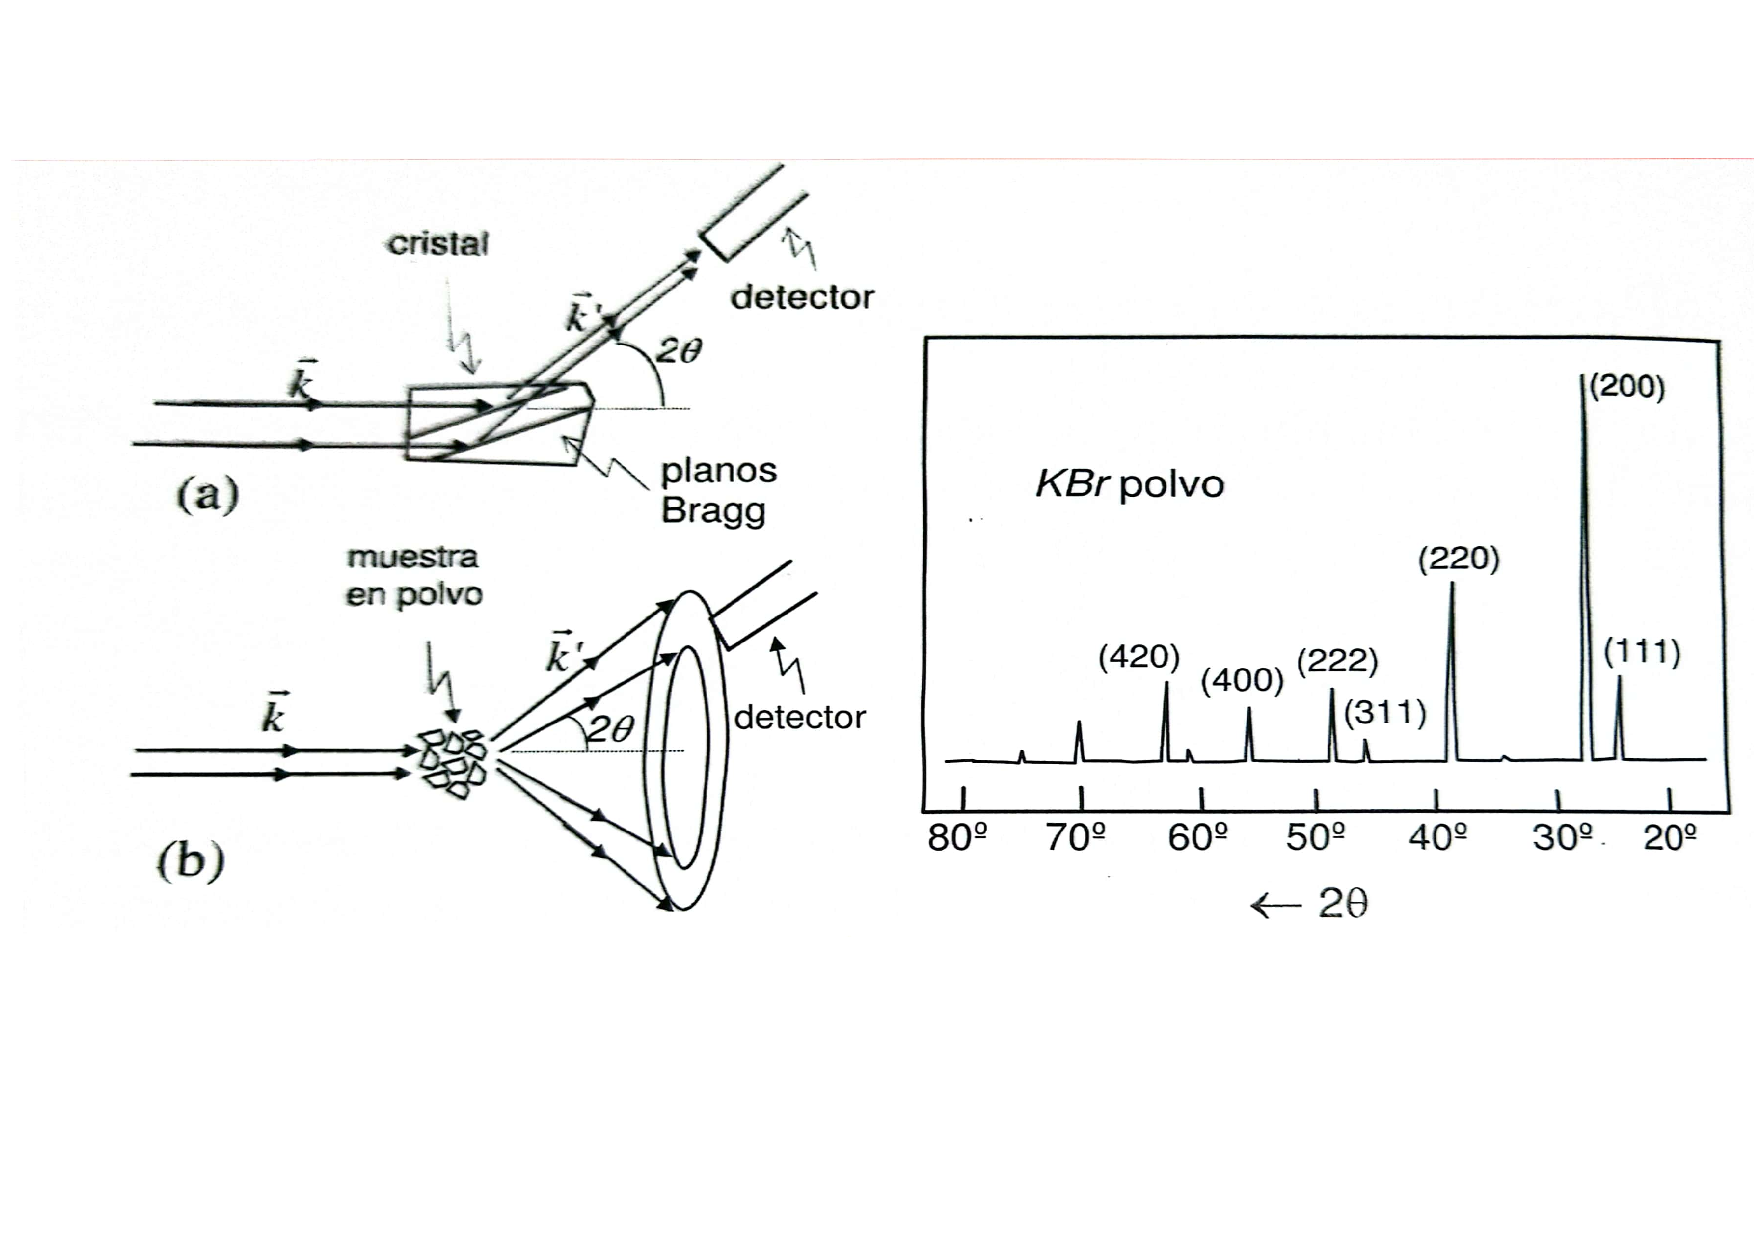
\includegraphics[scale=0.35]{Cuerpo/Ch_02/Fotos_libro 8.pdf}
    \caption{Esquemas de dos métodos de difracción (cristal rotatorio y polvo) y ejemplo de difractrograma que se obtiene.}
    \label{Fig:02-08}
\end{figure}

Una pregunta que nos podemos hacer es: ¿Cómo podemos diferenciar, si solo obtenemos los picos de difracción, las reglas de selección o la estructura de nuestro cristal? Existen dos formas. La primera, la más sencilla, es usando la siguiente ecuación:

\begin{equation}
    \frac{\sin \theta_2}{\sin \theta_1} = \frac{\sqrt{h_2^2+l_2^2+k_2^2}}{\sqrt{h_1^2+l_1^2+k_1^2}}
\end{equation}
En un primer lugar calculamos los senos cocientes de nuestros valores experimentales, colocando el más pequeño de ellos en el divisor. Así obtendremos un conjunto de números dados por $\{ \sin(\theta_1)/\sin(\theta_1)$, $\sin(\theta_2)/\sin(\theta_1)$, $\sin(\theta_3)/\sin(\theta_1) \}$... reales y mayores que uno. Debido a las reglas de selección de cada estructura, podremos hacer lo mismo con el cociente de las ternas. Colocando en la parte inferior la primera terna posible de la estructura (en el caso de la \sc \ el (100), en el caso de la \bcc \ la (110), en el de la \fcc \ la (111)), y colocando arriba las posibles ternas que permite la estructura, podremos obtener un conjunto de valores para cada estructura. Ahora solo queda comparar y ver cuales son los valores que más coinciden. Si el conjunto del seno tiene valores similares a las del conjunto de la \fcc, pues tendremos que dicho cristal es muy probable que tenga una estructura parecida. \\

Otra manera es realizar una tabla, asociando a cada uno de los ángulos un valor de la terna y ver cual es la que mas se acerca. Lógicamente este es un modelo experimental, y habrá diferencias, pero funciona correctamente.  \\

Tanto la falta de monocromaticidad como de paralelismo del haz incidente contribuyen a ensanchar los máximos. También, los defectos cristalinos afectan a los difractogramas; así la presencia de dislocaciones afecta a la anchura de los máximos de difracción de modo que su análisis se emplea, por ejemplo, para el estudio de defectos de los metales trabajados en frío. La temperatura, que genera vibraciones alrededor de las posiciones de equilibrio, no contribuye sin embargo a ensanchar los picos sino a disminuir su intensidad. Esto se entiende porque a mayor temperatura, en cualquier instante, menos átomos hay en las posiciones regulares (de equilibrio) y, por otro lado, la contribución de los átomos desviados en una determinada dirección, que generaría cambio en el haz difractado, es anulado por los que están desplazados en el sentido opuesto. 
    
\begin{figure}[h!] \centering
    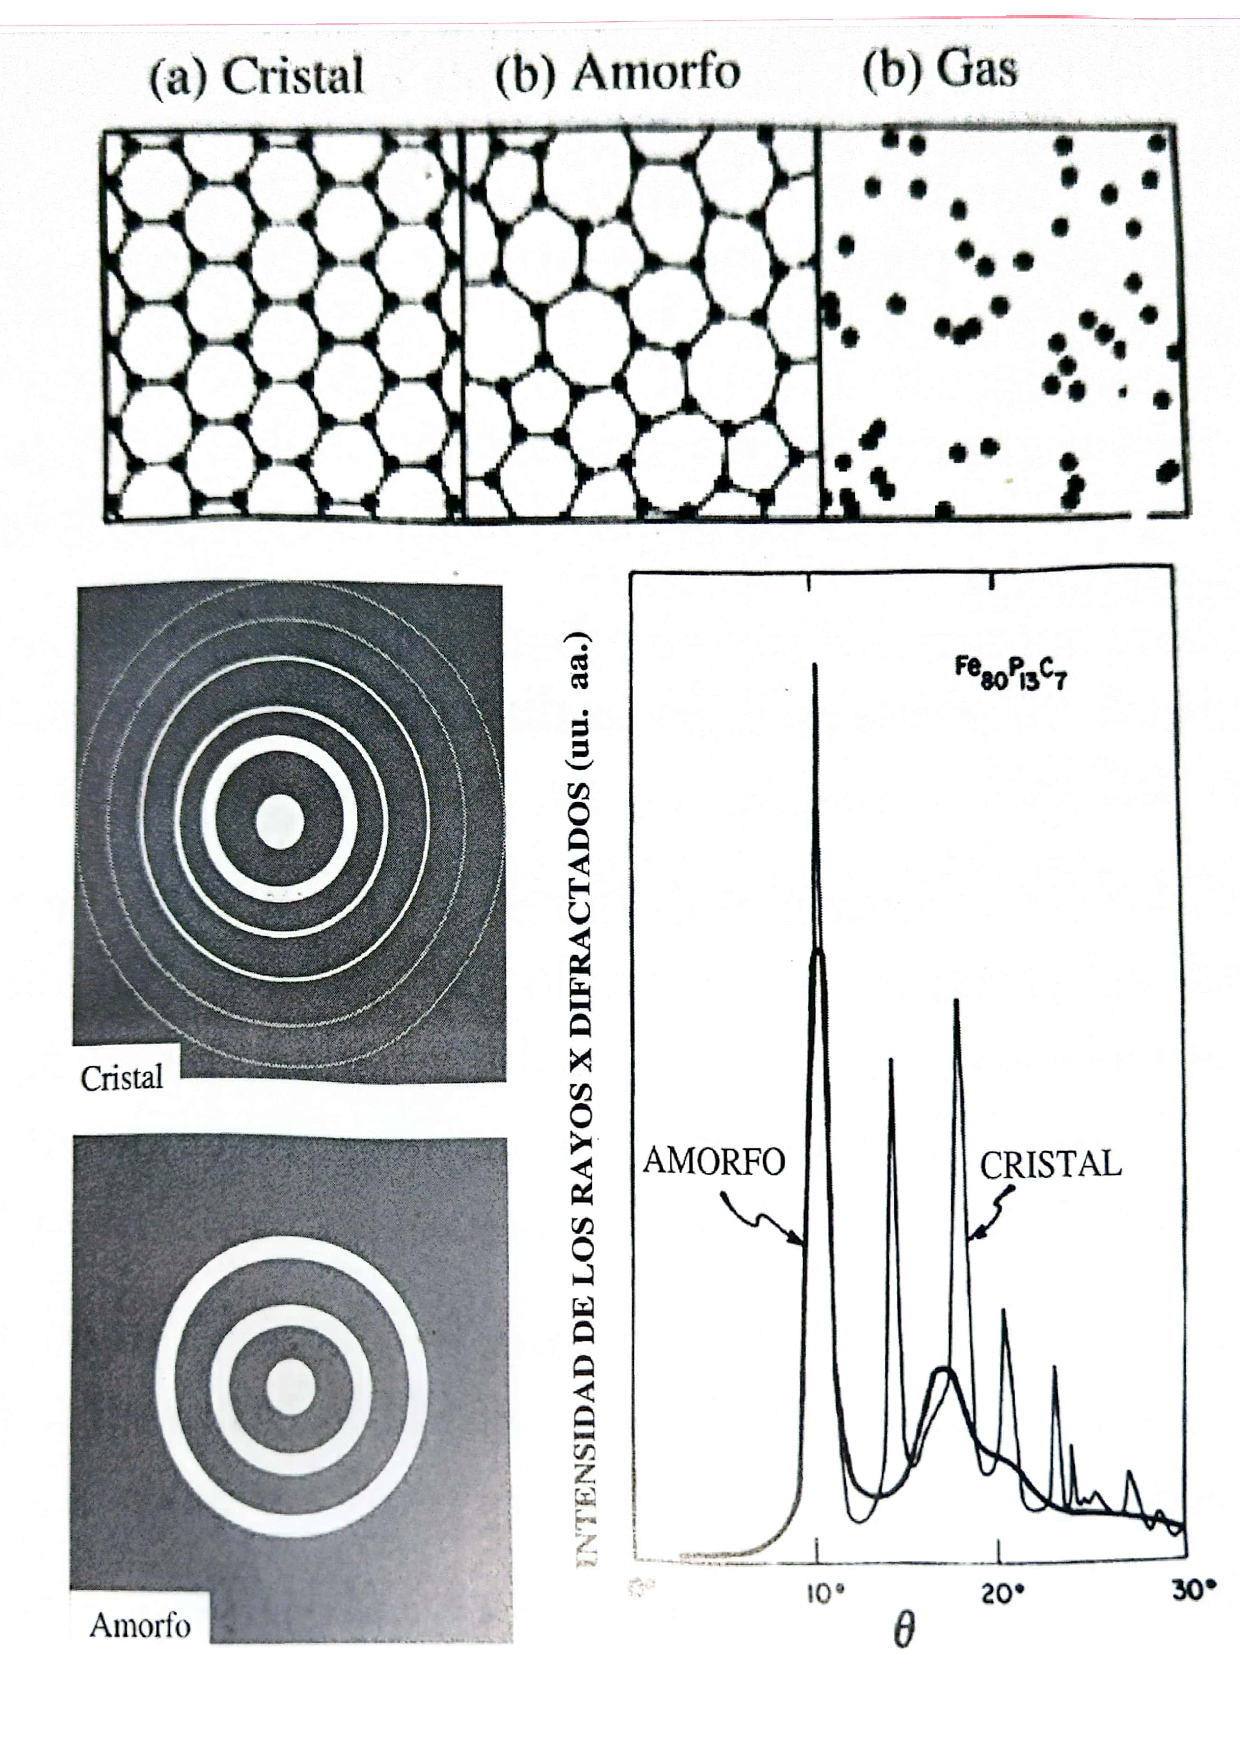
\includegraphics[scale=0.40]{Cuerpo/Ch_02/Fotos_libro 9.pdf}
    \caption{Efecto del desorden atómico en la difracción de rayos x.}
    \label{Fig:02-09}
\end{figure}

Es interesante hacer notar que la existencia de interferencia constructiva de los $N$ átomos de un cristal ($\sim 10^{28} \text{m}^{-23}$) es posible sólo gracias a que éstos están en posiciones regulares, es decir, están \textit{ordenados}. Que el orden está estrechamente asociado a la existencia de máximos de difracción lo muestra la figura \ref{Fig:02-08} donde se ve la correspondencia entre el orden espacial limitado de los materiales que se denominan amorfos con su espectro de difracción. Aquí la existencia de los dos picos de difracción a bajo ángulo está asociada al orden de corto alcance (primeros vecinos) característico de estos materiales.












